% imports
\documentclass[titlepage,twoside]{article}
\usepackage[utf8]{inputenc}
\usepackage[a4paper, total={16cm, 23cm}, top=3.5cm]{geometry}
\usepackage[dvipsnames]{xcolor}
\usepackage{
    amsmath,
    amssymb,
    amsthm,
    fancyhdr,
    siunitx,
    bm,
    lipsum,
    standalone,
    tikz,
    booktabs,
    enumitem,
    array,
    float,
}
\usepackage[colorlinks=true, allcolors=linkcolor]{hyperref}
\usepackage[nameinlink]{cleveref}
\usepackage[
    backend=biber,
    bibstyle=ext-authoryear,
    citestyle=ext-authoryear-comp,
    sorting=nyt,
    uniquename=false,
    maxbibnames=99,
    giveninits=true,
    sortcites=false,
]{biblatex}

% bibliographic options
\DeclareFieldFormat[article]{volume}{\mkbibbold{#1}}
\DeclareFieldFormat[article]{number}{\mkbibparens{#1}}
\DeclareFieldFormat[article]{pages}{#1}
\renewcommand*{\volnumdelim}{}
\renewbibmacro{in:}{}
\addbibresource{references.bib}
\DeclareFieldFormat{titlecase:title}{\MakeSentenceCase*{#1}}
\newrobustcmd*{\citefirstlastauthor}{%
    \AtNextCite{\DeclareNameAlias{labelname}{given-family}}\citeauthor
}

% ref options
\crefname{section}{\S}{\S\S}
\crefname{subsection}{\S}{\S\S}
\crefname{equation}{}{}
\crefname{figure}{Figure}{Figures}
\newcommand\crefrangeconjunction{--}
\def\equationautorefname~#1\null{(#1)\null}
\numberwithin{equation}{section}
\definecolor{linkcolor}{RGB}{51, 54, 142}

\makeatletter
\patchcmd{\math@cr@@@align}{\cr}{\global\let\df@label\@empty\cr}{}{}
\makeatother

% page style options
\setlength{\oddsidemargin}{0cm}
\setlength{\evensidemargin}{0cm}
\pagestyle{fancy}
\fancyhead[LE,RO]{\bfseries\thepage}
\renewcommand{\sectionmark}[1]{\markboth{\MakeUppercase{\thesection.\ #1}}{}}
\fancyhead[RE,LO]{\bfseries\nouppercase{\leftmark}}
\fancyfoot{}

\renewcommand{\headrulewidth}{0.5pt}
\setlength{\headheight}{15pt}
\setlength\parindent{0pt}
\setlength\parskip{6pt}

% math macros
\renewcommand{\d}[1]{\mathrm{d}#1}
\newcommand{\diff}[2]{\frac{\mathrm{d} #1}{\mathrm{d} #2}}
\newcommand{\ddiff}[2]{\frac{\mathrm{d}^2 #1}{\mathrm{d} {#2}^2}}
\newcommand{\pdiff}[2]{\frac{\partial #1}{\partial #2}}
\renewcommand\vec{\bm}
\newcommand{\uvec}[1]{\vec{\hat{#1}}}
\newcommand{\grad}{\vec{\nabla}}
\newcommand{\prandtl}{\ensuremath{\mathrm{Pr}}}
\newcommand{\rayleigh}{\ensuremath{\mathrm{Ra}}}
\newcommand{\nusselt}{\ensuremath{\mathrm{Nu}}}
\renewcommand{\bar}[1]{\mkern 1.5mu\overline{\mkern-1.5mu#1\mkern-1.5mu}\mkern 1.5mu}

% text macros
\newcommand{\rb}{Rayleigh-B\'{e}nard}

\begin{document}
\begin{titlepage}
\vfill~

\begin{center}
    {\Huge \textbf{%
        Novel parametrisation techniques in weather and climate modelling and
        their evaluation using simpler analogue models
    }} \\
    \vspace{0.75cm}
    {\Large\textbf{Thomas D. Schanzer}} \\
    \vspace{6pt}
    {\large Supervisor: Prof. Steven Sherwood} \\
    \vspace{0.75cm}
    {\large%
        School of Physics

        Climate Change Research Centre and
        ARC Centre of Excellence for Climate Extremes

        University of New South Wales, Sydney, Australia
    }
\end{center}
\vfill
\begin{center}
{\large\textbf{Abstract}}

\begin{minipage}{13cm}
    Text
\end{minipage}
\end{center}
\vfill
\end{titlepage}

\clearpage
\tableofcontents

\clearpage
\pagestyle{fancy}
\thispagestyle{fancy}

\section{Introduction and background} \label{sec:intro}
\subsection{The necessity of parametrisation}
% Broad introduction of weather/climate prediction and fluid equations
The primary task of general circulation models (GCMs) for Earth's weather and
climate is to simulate the dynamics of the atmosphere and ocean, which are
governed by the Navier-Stokes equations. The algorithm chosen to solve these
partial differential equations is known as a model's \emph{dynamical core}
\parencite{mcfarlane2011}. Since analytical solutions to the equations do not
exist, the dynamical core necessarily approximates the continuous equations
with finite-dimensional, exactly solvable alternatives using one of several
possible discretisation schemes (e.g., the finite difference, finite element,
finite volume and spectral methods) \parencite{christensen2022}. In practice,
this usually involves representing the prognostic variables (i.e., those that
affect the evolution of the flow) with sets of discrete samples in space and
time, whose resolution is constrained by the available computing resources. The
unavoidable consequence of discretisation is the loss of information about
processes occurring on spatial and temporal scales smaller than the
corresponding sampling intervals. These processes are said to be
\emph{unresolved}.

% why we need parametrisation: nonlinearity
It is tempting to na\"{i}vely accept the loss of fine-scale information as a
necessary sacrifice and hope the dynamical core will still make accurate
predictions for the larger, resolved scales. Unfortunately, this too is
impossible due to the \emph{nonlinearity} of the governing equations. The
reason for this may be seen by considering linear differential equations as a
counterexample. If the governing equations were linear, they would allow
arbitrary superpositions of solutions, meaning that any given solution could be
partitioned into high- and low-frequency components, themselves also solutions.
One would thus have the freedom to solve for the low-frequency components alone
without compromise. This property may be understood more formally using the
Fourier transform, defined for a function $f$ of space and time by
\[
    \tilde{f}(\omega, \vec{k})
        = \int \d{t}\,\d^3{x}\, e^{i(\vec{k} \cdot \vec{x} - \omega t)}
        f(t, \vec{x}),
\]
which reduces any linear differential equation to an algebraic equation
relating the frequency $\omega$ to the wave vector $\vec{k}$. Each wavenumber
component of the initial state propagates trivially according to its own
time dependence $e^{-i(\vec{k} \cdot \vec{x} - \omega(\vec{k}) t)}$,
\emph{independently of the other components}. If the equations of fluid
dynamics were linear, one could safely neglect the fine-scale dynamics because
they would have no influence on the coarse scales. In reality, the equations
are nonlinear cannot be solved by Fourier transform.

The consequence of the nonlinearity of the equations governing atmospheric and
oceanic flows is, therefore, a coupling of the resolved coarse scales to the
unresolved fine scales \parencite{mcfarlane2011}.
% justification via Reynolds averaging
This fact may be demonstrated more explicitly by applying so-called
\emph{Reynolds averaging} to the equations \parencite{christensen2022}.
Reynolds averaging decomposes each field $q$ into the sum of a coarse-grained
(in space or time) or statistical-ensemble-averaged field $\bar{q}$ and a
perturbation $q'$. Note that $\bar{q'} = 0$ by definition. The coarse-graining
operation is assumed to be linear, commute with differentiation and satisfy
$\bar{\bar{p} q} = \bar{p} \bar{q}$ for any two fields $p$ and $q$
\parencite{monin2007}. Following the example given by
\textcite{christensen2022}, consider the incompressible Navier-Stokes
equations, which have the general form
\begin{align*}
    \pdiff{u_i}{t} + u_j \pdiff{u_i}{x_j} &= \sum f_i, \\
    \pdiff{u_i}{x_i} &= 0
\end{align*}
where $u_i$ are the components of the velocity, $x_i$ are the
coordinates and $f_i$ are various forces per unit mass. Summation over repeated
indices is implied. Applying the decomposition and coarse-graining both sides
of the equations yields
\begin{alignat*}{2}
    && \pdiff{}{x_i} \left( \bar{u_i} + u_i' \right) &= 0 \\
    \Rightarrow & \qquad &
        \pdiff{\bar{u_i}}{x_i}
        + \underbrace{\pdiff{\bar{u_i'}}{x_i}}_{=0} &= 0 \\
    \Rightarrow & \qquad &
        \pdiff{\bar{u_i}}{x_i} = \pdiff{u_i'}{x_i} &= 0
\end{alignat*}
and
\begin{alignat*}{2}
    && \sum \bar{f_i} &=
        \bar{\pdiff{}{t} \left( \bar{u_i} + u_i' \right)}
        + \bar{\left( \bar{u_j} + u_j' \right)
        \pdiff{}{x_j} \left( \bar{u_i} + u_i' \right)} \\
    &&&=
        \pdiff{\bar{u_i}}{t}
        + \underbrace{\pdiff{\bar{u_i'}}{t}}_{=0}
        + \bar{u_j} \pdiff{\bar{u_i}}{x_j}
        + \bar{u_j} \underbrace{\pdiff{\bar{u_i'}}{x_j}}_{=0}
        + \underbrace{\bar{u_j'}}_{=0} \pdiff{\bar{u_i}}{x_j}
        + \bar{u_j' \pdiff{u_i'}{x_j}} \\
    &&&=
        \pdiff{\bar{u_i}}{t} + \bar{u_j} \pdiff{\bar{u_i}}{x_j}
        + \pdiff{\bar{u_i' u_j'}}{x_j}
        - \bar{u_i' \underbrace{\pdiff{u_j'}{x_j}}_{=0}} \\
    \Leftrightarrow & \qquad &
        \pdiff{\bar{u_i}}{t} + \bar{u_j} \pdiff{\bar{u_i}}{x_j}
        &= \sum \bar{f_i} - \pdiff{\bar{u_i' u_j'}}{x_j}.
\end{alignat*}
The physical meaning of this last equation is that the evolution of the
coarse-grained velocity field depends not only on itself and the coarse-grained
forces, but also on the perturbations via $\bar{u_i' u_j'}$, which does not
necessarily vanish. This dependence is a consequence of nonlinearity.

The theoretical discussion in this section establishes that physical processes
occurring at one place in the spectrum of temporal and spatial scales are
coupled to all the other processes in the spectrum \parencite{franzke2015}. In
particular, to ignore the effect of processes not explicitly resolved in
numerical models would introduce unacceptable systematic biases, or errors, in
the model forecasts. GCMs therefore require parametrisation schemes to estimate
the effects of unresolved processes as functions of the available large-scale
information (and the parameters of these functions must be chosen
appropriately---hence the name ``parametrisation'').


\subsection{Mathematical formulation of the parametrisation problem}%
\label{sec:math}
In order to make any progress on the parametrization problem, it is necessary
to formalise the notion of estimating the ``effects'' of unresolved processes.
I will describe the general approach, which is well-established \parencite[see,
e.g.,][]{hasselmann1976,palmer2001,demaeyer2018,brajard2021}, while
acknowledging possible alternative conventions where they exist.

The Earth system may be considered as a dynamical system whose exact evolution
is governed by equations of the form
\begin{equation} \label{eqn:truth}
    \diff{\vec{z}}{t} = \vec{F}(\vec{z},t),
\end{equation}
where the vector $\vec{z}$ contains all the variables needed to fully specify
the state of the system and $\vec{F}$ is a nonlinear differential operator. One
then employs a change of variables $\vec{z} \to (\vec{x},\vec{y})$, where
$\vec{x}$ contains the information or variables that are explicitly resolved by
the model being studied and $\vec{y}$ contains the unresolved, `sub-grid'
information or variables. Practically, $\vec{x}$ and $\vec{y}$ can be thought
of as projections of the full state $\vec{z}$ onto lower-dimensional
subspaces \parencite{brajard2021}. Alternatively (and more concretely),
$\vec{x}$ can be obtained by averaging the original variables over several
adjacent grid points, with $\vec{y}$ being the corresponding residuals
\parencite{zacharuk2018,alcala2021}.

In principle, the change of variables splits \cref{eqn:truth}
into two parts
\begin{align*}
    \diff{\vec{x}}{t} &= \vec{G}(\vec{x},\vec{y},t), \\
    \diff{\vec{y}}{t} &= \vec{H}(\vec{x},\vec{y},t)
\end{align*}
that (still exactly) describe the coupled evolution of the resolved and
unresolved variables via nonlinear differential operators $\vec{G}$ and
$\vec{H}$. The goal of parametrisation is now to derive a new system of
equations
\begin{equation} \label{eqn:reduced_model}
    \diff{\tilde{\vec{x}}}{t} = \tilde{\vec{G}}(\tilde{\vec{x}},t)
\end{equation}
whose solution $\tilde{\vec{x}}(t)$ approximates the true $\vec{x}(t)$ as well
as possible without explicitly modelling $\vec{y}(t)$. The measure used to
compare $\tilde{\vec{x}}$ and $\vec{x}$ depends on the intended function of the
parametrised model; weather forecasting applications that prioritise short-term
predictive skill might call for minimisation of the root-mean-square error
(RMSE), while climate prediction would be more concerned with the closeness of
their probability distributions (including both mean and extreme values).

Before proceeding, it is important to note two assumptions that are implicitly
made in writing down \cref{eqn:reduced_model}. The first is that
$\tilde{\vec{G}}$ is a \emph{deterministic} function of $\tilde{\vec{x}}$. The
second is that $\tilde{\vec{G}}$ depends only on the value of $\tilde{\vec{x}}$
at time $t$ and not earlier times (that is to say, the parametrisation is
\emph{memoryless}. Recent research has shown that relaxing these assumptions
has the potential to greatly improve the accuracy and reliability of the
parametrised model, and this will be discussed in detail in
\cref{sec:novel,sec:simple}. However, for the purpose of this basic
introduction, I will temporarily follow the traditional approach and retain
these assumptions.

There is more than one possible interpretation of $\tilde{\vec{G}}(\vec{x},t)$
and its relationship to $\vec{G}(\vec{x},\vec{y},t)$. \textcite{hasselmann1976}
describes $\tilde{\vec{G}}(\vec{x},t)$ as an ensemble average of
$\vec{G}(\vec{x},\vec{y},t)$, taken over the distribution of all $\vec{y}$ that
are possible for a given $\vec{x}$, i.e.
\begin{equation*}
    \tilde{\vec{G}}(\vec{x},t)
        = \langle \vec{G}(\vec{x},\vec{y},t) \rangle_{\vec{y}}.
\end{equation*}
\textcite{demaeyer2018} instead assert that the ultimate goal of
parametrisation is to literally approximate $\vec{y}$ as a function
$\vec{\xi}(\vec{x})$, in which case
\begin{equation*}
    \tilde{\vec{G}}(\vec{x},t)
        = \vec{G}(\vec{x},\vec{\xi}(\vec{x}),t).
\end{equation*}
In practice, $\vec{G}(\vec{x},\vec{y},t)$ usually separates into a known
resolved part $\vec{D}(\vec{x},t)$ independent of $\vec{y}$ and an unresolved
coupling term $\vec{C}(\vec{x},\vec{y},t)$. It then suffices to approximate
only the unresolved part by a parametrisation $\vec{P}(\vec{x}, t)$ using one
of the above methods, so that the parametrised model reads
\begin{equation} \label{eqn:parametrised_model}
    \diff{\tilde{\vec{x}}}{t}
        = \vec{D}(\tilde{\vec{x}},t) + \vec{P}(\tilde{\vec{x}}, t).
\end{equation}


\subsection{Physical processes requiring parametrisation}
% spectrum of scales and implications of cross-interaction
% Examples of processes requiring parametrisation
Following the broad theoretical argument in the previous sections, I now turn
to concrete examples of processes that are often represented by
parametrisations, restricting the discussion to atmospheric processes for
brevity. This section will give a basic introduction to each process, its
effect on the larger-scale behaviour of the climate system and the role of its
corresponding parametrisation scheme. The purpose of these examples is to
provide real-world context and motivation for current parametrisation research
in more idealised settings, which will form one of the main topics of this
review.

\emph{Cloud microphysics} parametrisations model the composition of clouds in
terms of the amount of water in the solid (e.g., hail), liquid (cloud droplets
and rain) and gaseous phases, and the rate of transitions between these phases.
Accurate representation of cloud formation and evolution is crucial for several
reasons. First, the interaction of clouds with solar and terrestrial radiation
has a major influence on the overall energy balance of the atmosphere
\parencite{mcfarlane2011}. Second, cloud water phase transitions lead to the
formation of precipitation, and are a source and sink of latent heat that
drives convection \parencite{mcfarlane2011}. Furthermore, the statistics of
cloud formation are linked to global temperatures in a feedback loop;
uncertainty in the sign and magnitude of this feedback effect is a major
contributor to uncertainty in the sensitivity of global temperatures to
increases in atmospheric CO$_2$ concentration \parencite{andrews2012,
christensen2022,stevens2013}. Microphysical processes occur on the spatial
scales of single water droplets and ice particles (of order
$\SIrange{e-6}{e-2}{\meter}$; \textcite{lamb2003}), among the smallest scales
in the atmosphere. All atmospheric models must parametrise the amount of cloud
water in each phase, the size distribution and concentration of liquid and ice
particles, and the resulting rate and type (rain, hail, snow, etc.) of
precipitation \parencite{christensen2022}.

\emph{Moist convection} encompasses vertical motions in the atmosphere that are
accompanied (and driven) by phase changes of water, and must be parametrised
when it occurs on sub-grid scales. Moist convection is generally triggered by
warming and moistening at low levels, which create convective instability, and
is manifested by narrow updrafts and downdrafts that can rarely be resolved
explicitly \parencite{mcfarlane2011}. Convection transports heat and moisture
vertically, removing the instability and generating storms where the condensed
water falls out as precipitation; more broadly, it is a key component of the
global atmospheric circulation in spite of its small spatial scale
\parencite{christensen2022}.

It should be noted that parametrisation also encompasses estimation techniques
for processes that are too complex to model exactly for reasons unrelated to
spatial and temporal resolution \parencite{mcfarlane2011}. A good example of
such a process is \emph{radiative transfer}. Air and its constituent gases, as
well as clouds, absorb, emit, reflect and/or scatter solar and terrestrial
radiation. This leads to differential heating and cooling that drives the
atmospheric circulation. While the theory of radiative transfer is understood
well enough to allow precise calculations in principle, the prohibitive
computational cost of such calculations necessitates a parametrisation based on
simplifying assumptions (the details of which are beyond the scope of this
review) \parencite{christensen2022}.


\subsection{Traditional solutions to the problem and their limitations}%
\label{sec:traditional}
With the examples of cloud microphysics, moist convection and radiative
transfer in mind, I now broadly review the traditional approaches used to
construct parametrisation schemes in practice. In particular, this section will
identify the key assumptions upon which many traditional schemes are founded,
and the circumstances under which the assumptions may be violated. This will
motivate research into novel approaches.

% conceptual model (examples)
A parametrisation scheme is traditionally constructed by formulating a
simplfied, easily solvable and deterministic conceptual model of the physical
process in question. The solution of this model is then used to estimate the
effect of the process on the coarse-scale state of the parent model, known as
the \emph{unresolved tendency} \parencite{mcfarlane2011}. For example, the
earliest convective parametrisation was developed by \textcite{manabe1965} and
simply assumed that the net effect of convection is to relax the vertical
structure of the atmosphere towards a neutrally stable state whenever it
becomes convectively unstable.
% motivate data-driven parametrisation here?
One obvious deficiency of simple conceptual models is that they cannot possibly
capture the full range of variability in the processes they simulate. One major
branch of modern parametrisation research therefore studies \emph{data-driven}
schemes that instead use observational or high-resolution simulated data to fit
empirical models for the unresolved processes, naturally capturing a wider
range of variability \parencite{christensen2022}. Data-driven parametrisation
will be discussed in much further detail in the next section.

% grid-box mean and scale separation
In general, a traditional parametrisation scheme aims to capture the net
unresolved tendency due to all occurrences of the unresolved process (e.g., all
convective updrafts and downdrafts) within each grid cell of the parent model.
A deterministic prediction of this type is valid when each grid cell contains
many independent realisations whose varying contributions may be expected to
yield a reliable average tendency. This requires a \emph{scale separation}
between the unresolved process and the resolution of the parent model. Scale
separation breaks down when model development and increases in available
computing resources allow simulations at resolutions approaching the previously
unresolved scales. In this case, knowledge of the coarse-scale state cannot be
expected to uniquely determine the unresolved tendency because the process is
only realised a few times in each grid cell. The resulting (seemingly) random
nature of the true unresolved tendency motivates stochastic treatments
\parencite{mcfarlane2011,christensen2022,berner2017}. These will be discussed
in the next section.

% closure, quasi-equilibrium -> memory
The conceptual models core to traditional parametrisations usually contain free
parameters that are determined from the coarse-scale model state using
additional assumptions called \emph{closures}. Closures often postulate a state
of quasi-equilibrium between the unresolved processes and their large-scale
environment, such as a balance between the accumulation of convective available
potential energy (CAPE) and its removal by convection, or between the
horizontal convergence of moisture at low levels and its convective transport
to higher levels \parencite{mcfarlane2011,christensen2022,palmer2019}. However,
there is no guarantee that such an equilibrium exists; in fact, it has been
demonstrated that the CAPE balance is violated by fluctuations on sub-diurnal
time scales \parencite{donner2003} and by midlatitude continental convection
\parencite{zhang2002}. Newer parametrisation schemes have allowed departures
from equilibrium by representing the unresolved processes in a prognostic
rather than diagnostic manner (i.e., allowing the processes to have their own
self-governing time dependence rather than calculating them from the
large-scale state at each time step independently of their values at the
previous step) \parencite{rio2019,berner2017}. This creates \emph{memory} or
\emph{latency} in the parametrised tendencies, meaning that the tendencies have
some nonzero response time when subjected to sudden changes in the large-scale
state. Memory will be discussed further in the next section.

% ISSUES
Parametrisation schemes commonly suffer from several other issues that I will
briefly address here.
% division of processes -> unification
Firstly, while the division of the general atmospheric dynamics into a set of
separately parametrised processes (microphysics, convection, etc.) is
physically motivated, it remains somewhat arbitrary because these processes,
strictly speaking, form a continuum without well-defined boundaries
\parencite{christensen2022,mcfarlane2011}. It is a goal of contemporary
research to unify the parametrisations as much as possible.
% universality
Secondly, given the importance of future climate projections, it is natural to
ask whether the parametrisation schemes that have been developed and tuned on
today's climate remain valid as the climate changes over decade- to
century-long simulations. This is a matter of particular concern for
data-driven parametrisations, since there is little reason to trust empirical
models once they are extrapolated beyond the range of the data originally used
to fit them \parencite{christensen2022}.
% conservation laws
Finally, unless very special care is taken, parametrisation schemes can cause
the parent model to violate known physical conservation laws (e.g., mass,
energy and momentum) \parencite{christensen2022}. Efforts to resolve this issue
are ongoing.


\clearpage
\section{Novel approaches to the parametrisation problem}%
\label{sec:novel}
% ongoing issues, processes will remain unresolved
Since the 1990s, the limitations identified in \cref{sec:traditional} have
prompted many to reconsider the principles upon which parametrisation schemes
are founded. The main advance has been the development of stochastic
parametrisations that incorporate random noise in the predicted tendencies.
More recently, others have approached the problem from an entirely new
direction, developing data-driven parametrisations that learn to predict the
tendencies empirically. This section will introduce the stochastic and
data-driven approaches in general terms while omitting the technical details of
individual implementations, the aim being to contextualise and motivate the
study of these approaches in more idealised frameworks in \cref{sec:simple}.
Other methods (such as superparametrisation) exist but are beyond the scope of
this review.


\subsection{Stochastic parametrisation and memory} \label{sec:stochastic}
The potential value of stochasticity for climate modelling was first
established by \textcite{hasselmann1976}, whose seminal paper sought to explain
the characteristics of long-term climate variability. Knowing that climate
depends on interactions between all components of the Earth system
(atmosphere, ocean, cryosphere, biosphere, etc.), \citeauthor{hasselmann1976}
argued that the effect of the more rapidly-evolving atmosphere on the other,
more slowly-varying components is that of a stochastic forcing. Owing to
their long response time, the slowly-varying components effectively integrate
this stochastic forcing, allowing long-term climate variability to be
characterised as a type of random walk process akin to the Brownian motion
of a massive particle in a fluid.

Further motivation for stochastic parametrisation in particular stems from the
need to reliably estimate uncertainties in weather forecasts and climate
projections. Weather forecasting centres typically propagate initial condition
uncertatinties (due to imperfect observations) through to the final forecast in
a Monte Carlo fashion, by initialising an ensemble of model runs with perturbed
initial conditions and measuring the spread of the resulting forecasts. It has
been observed that deterministic models produce systematically under-dispersed
ensembles that fail to span the range of actual weather outcomes, indicating
that these models are failing to capture additional sources of variability
\parencite{palmer2005,berner2017,palmer2019}. Knowing that poor scale
separation and departures from quasi-equilibrium should preclude deterministic
relationships between unresolved tendencies and the large-scale state (see
\cref{sec:traditional}), it should seem highly likely that deterministic
parametrisation contributes to this deficiency.

% should this go at the beginning of the subsection so we get the point quicker?
The principle of stochastic parametrisation is, therefore, that unresolved
tendencies should be randomly sampled from an appropriate distribution at each
point in space and time, not simply set to the mean of the distribution
\parencite{franzke2015}. This choice has now been theoretically justified using
statistical mechanical arguments; most notably,
\textcite{wouters2012,wouters2013} showed that, assuming a weak coupling to the
resolved variables, the effect of unresolved dynamics should be parametrised by
a combination of deterministic and stochastic terms, as well as a
\emph{non-Markovian} memory term depending on the past states of the resolved
variables.

The simplest and earliest approach to stochastic parametrisation is the method
of \emph{stochastically perturbed parametrisation tendencies} (SPPT), which
takes an existing deterministic parametrisation and randomly scales its output
with a multiplicative noise field \parencite{palmer2019,christensen2020}.
Re-using the notation of \cref{sec:math}, an SPPT model for the resolved
variables $\vec{x}$ takes the form
\begin{equation*}
    \diff{\vec{x}}{t}
        = \vec{D}(\vec{x},t)
        + [I + \operatorname{diag}(\vec{e})] \vec{P}(\vec{x}, t),
\end{equation*}
where $\vec{P}$ is the existing deterministic parametrisation, $\vec{e}$ is a
mean-zero random vector with the same length as $\vec{x}$ and $I$ is the
identity matrix. The choice of multiplicative (and thus inherently
state-dependent) rather than additive noise is intuitively motivated by the
expectation that variability in the effect of unresolved processes should be
greatest when those processes are most active \parencite{franzke2015}.
\textcite{christensen2020} performed a comparison of high-resolution
simulations to parametrised single-column model output which justified the use
of multiplicative perturbations.

In GCMs, where the variables being modelled have spatial dependence, the
multiplicative perturbation takes the form of a random \emph{field}
$e(x,y,t)$. It has been argued that this random field should be spatially and
temporally correlated (in contrast to uncorrelated ``white'' noise) in order to
emulate the organisation of unresolved processes on larger scales and their
persistence in time \parencite{christensen2022,franzke2015}. In particular,
perturbations that explictly depend on their own past values constitute a type
of memory, albeit distinct from the memory term advocated by
\textcite{wouters2012,wouters2013}, which would instead couple the
perturbations to the past values of the large-scale variables.

Stochastic parametrisations have several known advantages over their
deterministic counterparts, and are now implemented in operational weather
forecast models. They have been found to remedy the aforementioned issues of
ensemble underdispersion and prediction unreliability
\parencite{palmer2005,berner2017}, and (as of 2009) even make the skill of
five-day forecasts comparable to that of deterministically parametrised two-day
forecasts \parencite{palmer2019}. Despite the zero-mean nature of the noise, it
has been shown that stochastic parametrisations can reduce systematic model
biases (``noise-induced drift''; \textcite{palmer2005}) and stabilise the
simulation of regime-based behaviour (such as the El Ni\~{n}o-Southern
Oscillation) in the climate system \parencite{berner2017}.

Reviewing the field, \textcite{palmer2019} identifies outstanding issues for
further research. The main concern is the lack of rigour in most stochastic
schemes; SPPT, for example, modifies existing deterministic schemes \emph{ad
hoc} rather than incorporating stochasticity \emph{ab initio} in the
development process. More objective approaches are yet to gain widespread
acceptance. This motivates both data-driven methods and further testing
using simpler dynamical systems where objectivity is more feasible.


\subsection{Data-driven parametrisation and machine learning}%
\label{sec:data_driven}
The fitting of predictive statistical models to data is, of course, ubiquitous
in the sciences, but attempts to use such models as parametrisation schemes and
couple them into fully fledged GCMs are a relatively new phenomenon---certainly
more so than stochastic parametrisations. The prerequisite for all data-driven
parametrisations is obviously training data: mathematically, an approximate
solution of \cref{eqn:truth} of sufficient accuracy and resolution to be
considered ``truth'' for the application at hand. Training data are typically
derived from high-resolution simulations, such as regional weather model runs
or large eddy simulations (LES). The other ingredient is the imperfect
low-resolution model that will later be augmented by parametrisation.

To generate an appreciation of how these data might be used to construct a
parametrisation in practice, I roughly follow the argument and notation of
\textcite{brajard2021}. Define a map $\mathcal{M}$ that takes each state
$\vec{z}(t)$ in the training dataset to the state $\vec{z}(t + \delta t)$ at
the next time step. Similarly, denote by $\mathcal{M}^\mathrm{r}$ the
low-resolution model (the superscript r meaning ``reduced''), which maps a
low-resolution state $\vec{x}(t)$ to a prediction for $\vec{x}(t + \Delta t)$,
where $\Delta t$ is not necessarily equal to $\delta t$ (usually larger). The
spaces of high- and low-resolution states, having different dimensions, may be
linked by an operator $\langle \cdot \rangle$ that projects high-resolution
states onto the low-resolution state space. Practically, the projection
operation is simply a coarse-graining of $\vec{z}$ by averaging values at
adjacent grid points to match the resolution of $\vec{x}$. Now, for each state
$\vec{z}$ in the training dataset, one may compute the difference
\begin{equation*}
    \vec{\epsilon}(\vec{z}) =
        \frac{
            \langle \mathcal{M}(\vec{z}) \rangle - \langle \vec{z} \rangle
        }{\delta t}
        - \frac{
            \mathcal{M}^\mathrm{r}(\langle \vec{z} \rangle)
            - \langle \vec{z} \rangle
        }{\Delta t}
\end{equation*}
between the coarse-grained true tendency (on the left) and the tendency
predicted by the coarse model when it sees the same state (on the right). This
is the unresolved tendency. Knowledge of $\langle \vec{z} \rangle$ alone does
not uniquely determine $\vec{\epsilon}$ because $\langle \mathcal{M}(\vec{z})
\rangle$ depends on the original $\vec{z}$. However, if one can fit a
statistical model $\vec{P}$ to the dataset of ($\langle \vec{z} \rangle$,
$\vec{\epsilon}$), then $-\vec{P}(\vec{x}(t)) \Delta t$ will be able to serve
as an estimate of the error incurred by the coarse model in predicting
$\vec{x}(t + \Delta t)$ given $\vec{x}(t)$. This motivates the construction of
a parametrised model $\mathcal{M}^\mathrm{p}$, defined by
\begin{equation*}
    \mathcal{M}^\mathrm{p}(\vec{x}) =
        \mathcal{M}^\mathrm{r}(\vec{x}) + \vec{P}(\vec{x}) \Delta t
\end{equation*}
that simply subtracts the estimated error at each time step of the coarse
model. In theory, the solution $\vec{x}(t)$ obtained by iteration of
$\mathcal{M}^\mathrm{p}$ will be more accurate than that obtained by
iteration of the unparametrised $\mathcal{M}^\mathrm{r}$.

The current method of choice for constructing $\vec{P}$ in weather and climate
modelling contexts is machine learning (ML). I will briefly introduce the key
concepts, strengths and weaknesses of ML, following \textcite{beucler2022}. ML
encompasses a broad class of algorithms that programmatically and autonomously
develop and apply rules for performing tasks, such as image classification,
removing the need for a human to explicitly program the rules. They do this
using supplied \emph{training data} that exemplify the task to be performed.
When it comes to data-driven parametrisation, the task is function
approximation or regression, and the relevant algorithms usually require a
training dataset of example inputs (i.e., coarse-scale variables)
\emph{labelled} with the desired outputs (i.e., unresolved tendencies). One
commonly-used class of algorithms called \emph{neural networks} consist of
layers of inter-communicating calculation nodes called neurons and learn to
approximate functions by optimising sets of weights associated with the
neurons. Another type of algorithm is the \emph{random forest}, which
approximates functions by passing the inputs through a series of nested
\texttt{if/else} decision trees.

The distinguishing advantage offered by ML data-driven parametrisations is
their ability to systematically capture complex relationships without relying
on artificially simplified physical models derived by humans
\parencite{irrgang2021,beucler2022}. In addition to constructing new
parametrisations from scratch, ML has been used to emulate the action of
existing parametrisation schemes in GCMs \parencite[e.g.,][]{gentine2018}.
These ML emulators have the potential to reduce the computational burden that
parametrisation usually imposes, leaving more resources for other tasks such as
calling the parametrisation scheme more frequently or increasing the model
resolution \parencite{beucler2022}. Furthermore, the ability to emulate
multiple existing schemes at once is a step towards unifying the
parametrisation of unresolved processes (a long-standing issue; see
\cref{sec:traditional}).

ML parametrisations are not without their issues; they are known to be prone to
overfitting and often cause their host models to become numerically unstable.
They are also, by their very nature, far more difficult to interpret than
traditional schemes. It is therefore very difficult to determine \emph{a
priori} whether or not they will continue to be valid in climate conditions
outside the bounds of their training datasets
\parencite{irrgang2021,beucler2022}. ``Interpretable'' or ``explainable'' ML is
an active area of research that aims to address these issues. Another active
research topic is ``physics-guided ML'', the aim of which is to augment ML with
known physical constraints and conservation laws that would otherwise be
violated \parencite[e.g.,][]{yuval2021}.


\clearpage
\section{Simple dynamical systems as testbeds for novel approaches}%
\label{sec:simple}
Historically, it has been common practice to develop and test new
parametrisation techniques using simpler dynamical systems that share the key
nonlinear, multi-scale and chaotic properties of the climate system. These
analogue systems provide testbeds where the parametrisation problem is more
tractable, avoiding the expense, effort and technicalities of fully-fledged
climate models. The simplicity of these systems also helps to ensure the
reproducibility of the results obtained. This section will review the progress
that has been made using simple analogue systems and argue that, considering
the outstanding issues identified in \cref{sec:intro,sec:novel}, further
research using these systems may yet be warranted. The relevant techniques for
constructing and testing parametrisation schemes in simple model frameworks,
and the remaining open questions, will be discussed in order to inform future
research.

% The most popular option is the so-called Lorenz '96 model, which will be
% addressed along with other ``toy'' models of its kind in \cref{sec:l96}.
% More recent work has used more sophisticated models of idealised fluid flows
% and will be discussed in \cref{sec:simple_fluid}.


\subsection{The Lorenz '96 system}
The Lorenz '96 model (henceforth L96) was proposed by eminent meteorologist
Edward N. Lorenz in a \citeyear{lorenz1995} paper \parencite{lorenz1995} on the
growth of errors in solutions of dynamical systems and the resulting limits of
predictability for those systems. \citeauthor{lorenz1995} proposed to mimic the
multi-scale nature of the climate system by coupling two dynamical systems with
different characteristic time scales. Following his notation, there is a
discrete set of ``slow'' variables $\{X_k\}_{k=1}^K$, each of which has an
associated discrete set of ``fast'' variables $\{Y_{j,k}\}_{j=1}^J$. The
indices of the slow variables are periodic ($X_{K+1} = X_1$ and $X_0 = X_K$)
and the sets of fast variables are arranged end-to-end so that $Y_{J+1,k} =
Y_{1,k+1}$ and $Y_{0,k} = Y_{J,k-1}$. The intuition is that the variables
represent samples of a field along a latitude circle, as shown in
\cref{fig:L96_diagram} (a reproduction of Figure 1 by \textcite{russell2017}).
The evolution of the system is governed by the ordinary differential equations
\begin{subequations} \label{eqn:l96}
\begin{align}
    \diff{X_k}{t}
        &= -X_{k-1} (X_{k-2} - X_{k+1}) - X_k + F
        - \frac{hc}{b} \sum_{j=1}^J Y_{j,k}, \\
    \diff{Y_{j,k}}{t}
        &= -cb Y_{j+1,k} (Y_{j+2,k} - Y_{j-1,k}) - c Y_{j,k}
        + \frac{hc}{b} X_k.
\end{align}
\end{subequations}
The constant $c \geq 1$ dictates the ratio of the time scale of the $Y$
variables to the time scale of the $X$ variables, $b$ the typical
magnitude of $X$ relative to $Y$, $h$ the strength of the coupling
between the two subsystems and $F$ the constant forcing applied to each
$X$ variable.

\begin{figure}[ht]
    \centering
    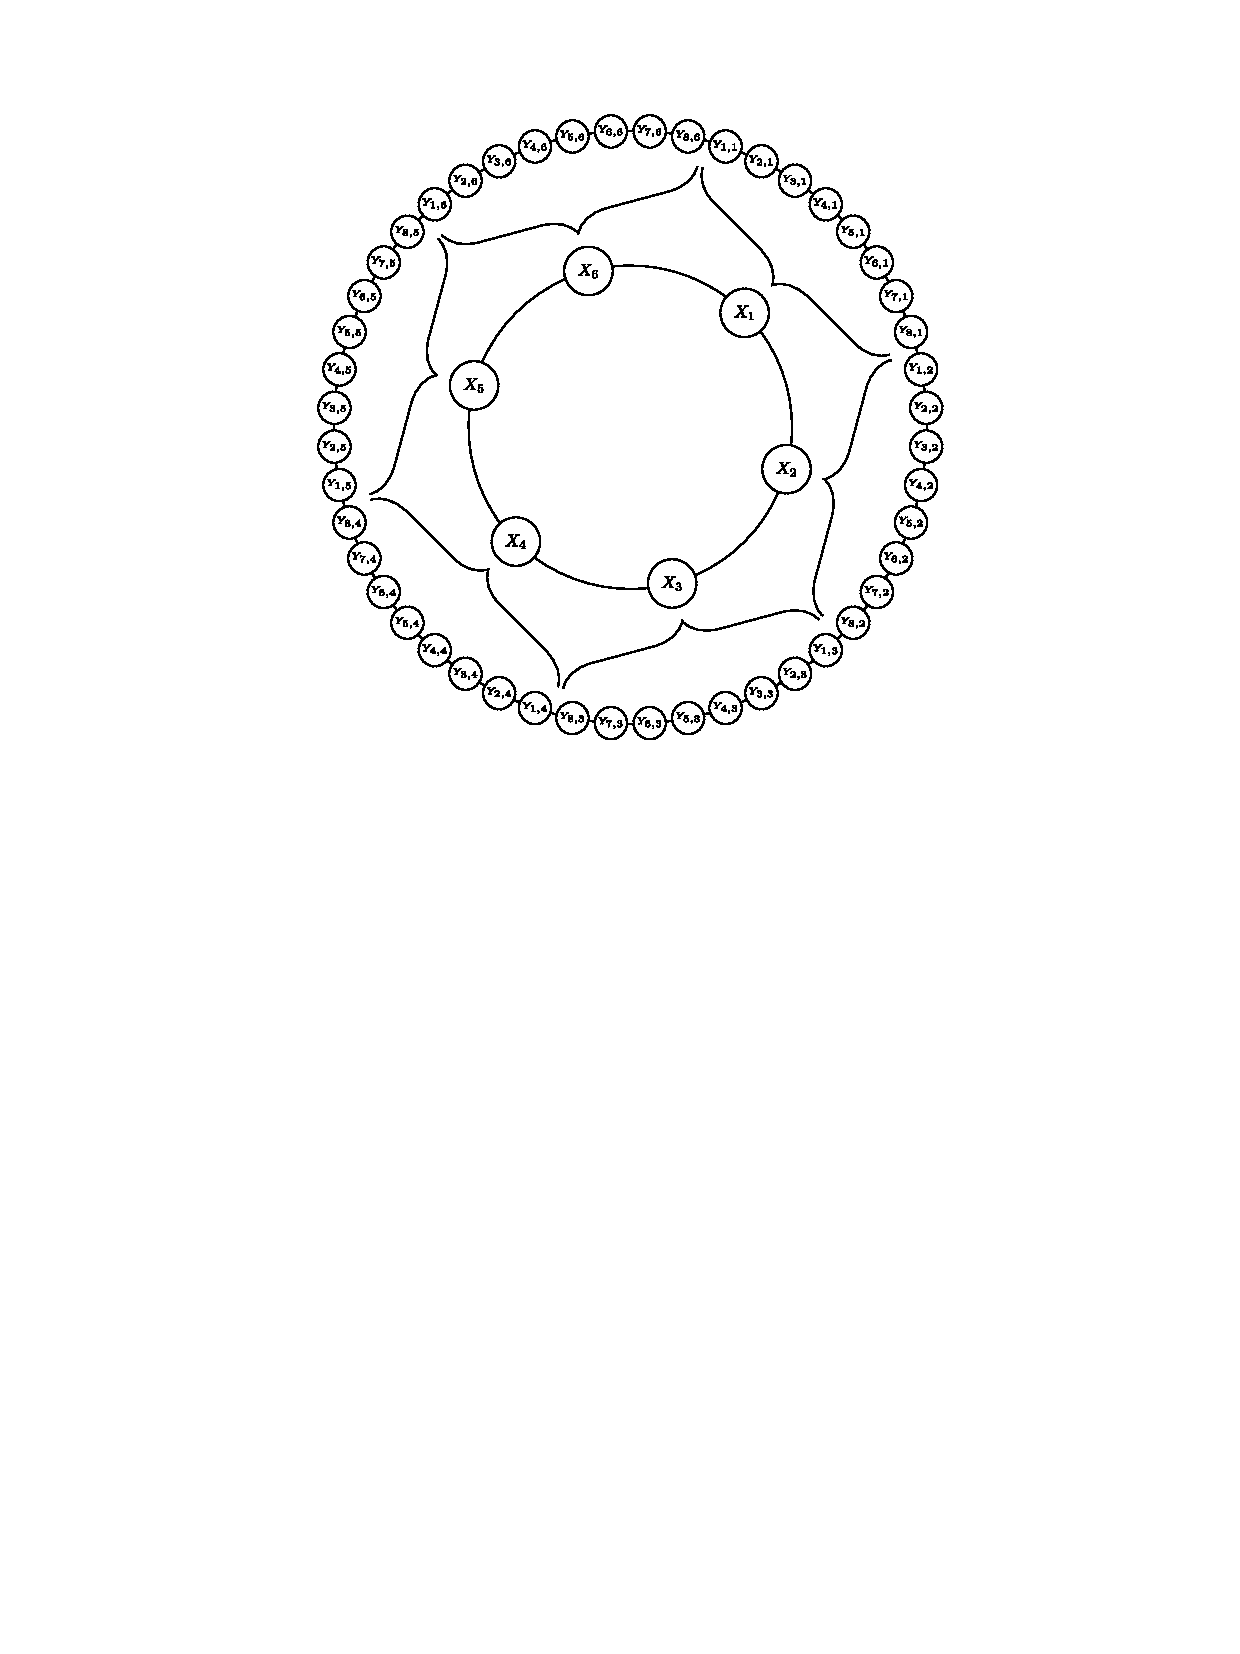
\includegraphics[width=0.7\linewidth]{figures/russell2017_L96_diagram.pdf}
    \caption{
        Illustration of the periodic arrangement of the L96 variables,
        with the slow variables $X_k$ arranged in a circle. Each slow variable
        is coupled to a neighbouring subset of the similarly arranged fast
        variables $Y_{j,k}$. Reproduced from \textcite{russell2017}, Figure 1.
    }
    \label{fig:L96_diagram}
\end{figure}

As discussed in \cref{sec:math}, the objective is to find $P_k(X_1, \dots, X_K)
\approx -(hc/b) \sum_{j=1}^J Y_{j,k}$ such that the solution of the
parametrised system
\begin{equation*}
    \diff{X_k}{t}
        = -X_{k-1} (X_{k-2} - X_{k+1}) - X_k + F + P_k(X_1, \dots, X_K)
\end{equation*}
approximates as accurately as possible the true $X_k$ obtained by solving
\cref{eqn:l96}. The simple form of L96 allows one to generate a training
dataset by numerically solving \cref{eqn:l96} and directly diagnosing the
unresolved tendency of $X_k$ as
\begin{equation} \label{eqn:l96_tendency}
    U_k(t) = \frac{X_k(t + \Delta t) - X_k(t)}{\Delta t}
        - \left[ -X_{k-1} (X_{k-2} - X_{k+1}) - X_k \right].
\end{equation}
As we shall see, it is usually assumed that $P_k$ depends only on $X_k$ (i.e.,
the parametrisation is \emph{local}) but may also depend on the value of $X_k$
at earlier times. The symmetry of \cref{eqn:l96} under shifts of the $k$ index
implies that all the $X_k$ have the same long-term statistics, so it suffices
to aggregate all the $U_k$ into a single training dataset and use the resulting
parametrisation for all the $X_k$ rather than constructing a separate
parametrisation for each variable.

\subsection{Statistical models} \label{sec:l96_statmodels}
Constructing a data-driven parametrisation scheme for L96 requires first
choosing the structure of the scheme and then using the training dataset to
find the optimal values of the associated free parameters. The simplest
structure, popularised in an influential paper by \textcite{wilks2005},
consists of a polynomial regression of $U$ against $X$ as a deterministic base,
modified by stochastic noise. Wilks' scatterplot of $U$ and $X$ and quartic
polynomial least-squares regression, shown in \cref{fig:wilks2005_regression},
confirm that such a structure is reasonable.

\begin{figure}[ht]
    \centering
    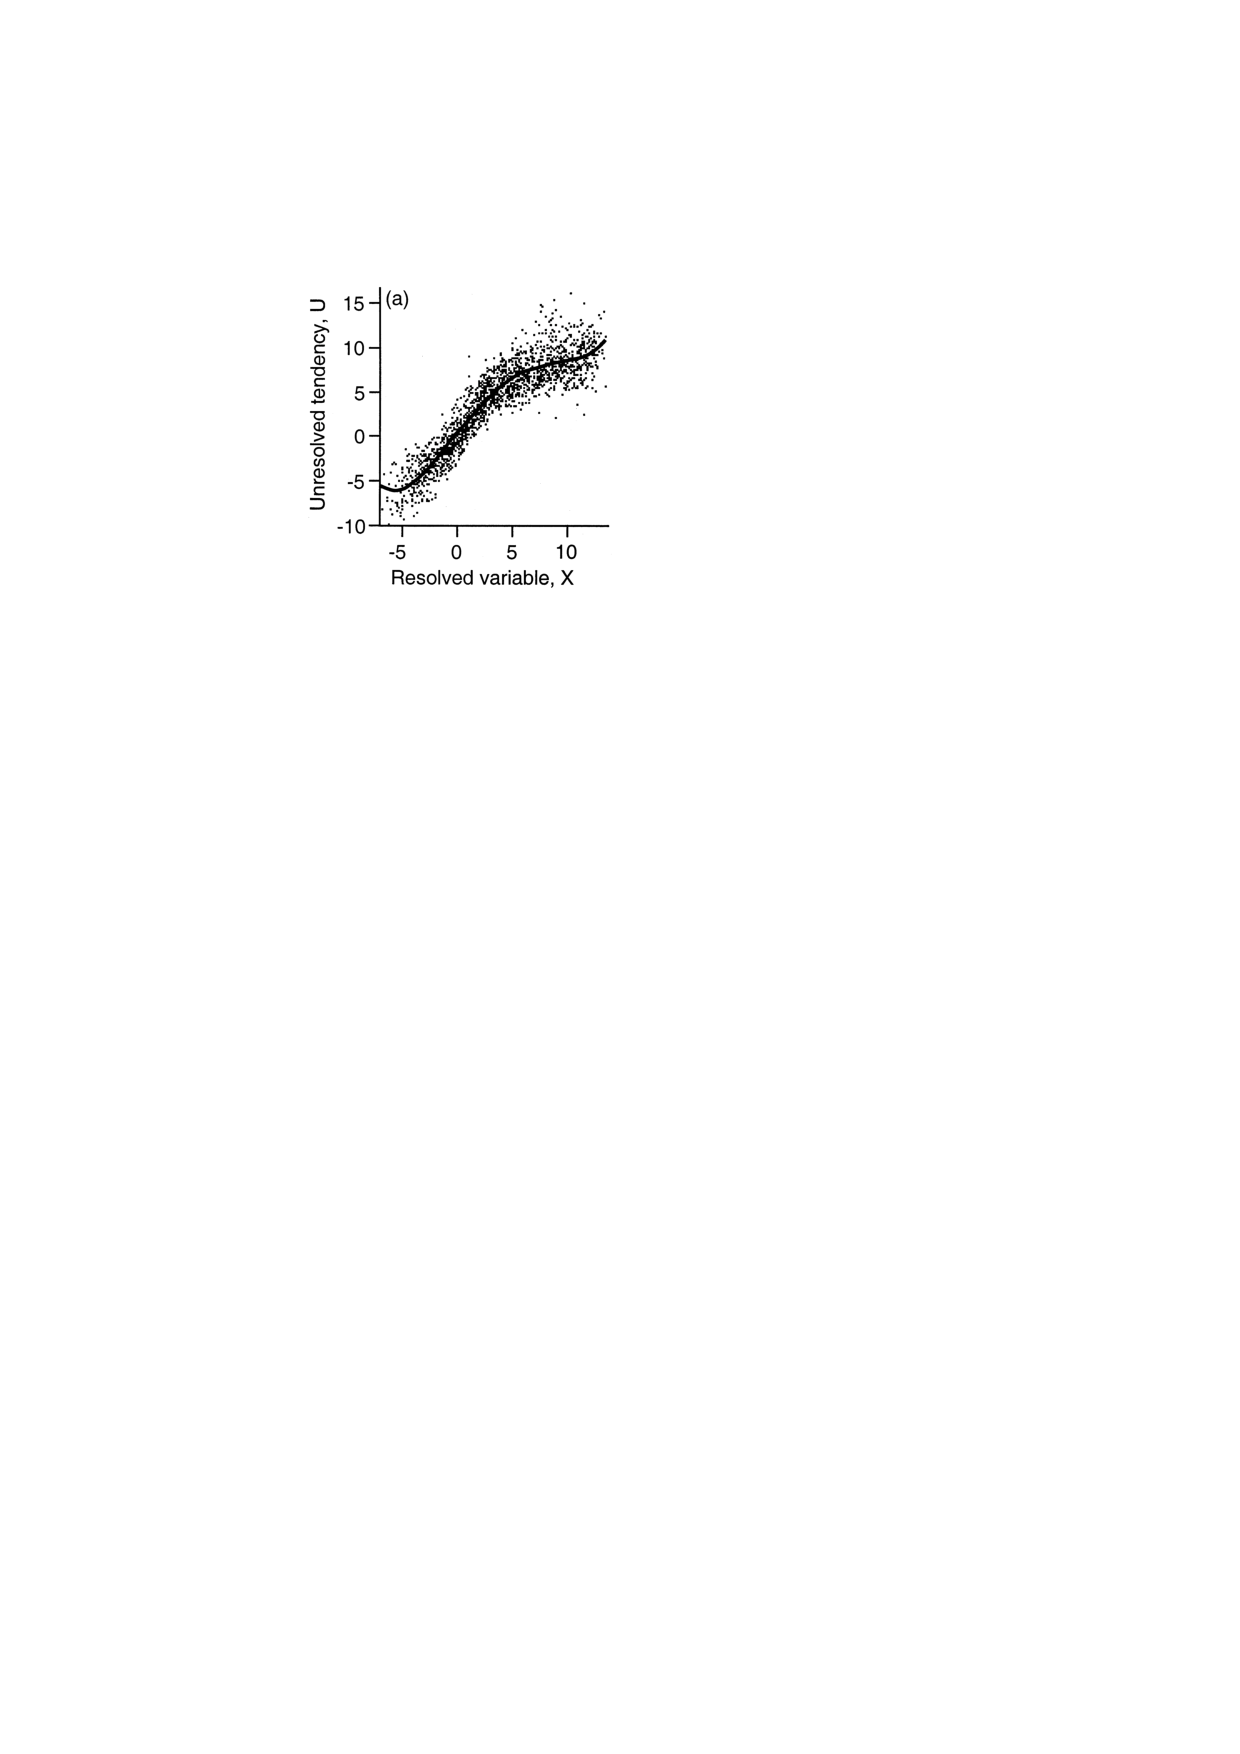
\includegraphics[width=0.3\linewidth]{figures/wilks2005_regression.pdf}
    \caption{
        Scatterplot of unresolved tendencies $U$ against large-scale variables
        $X$ in L96 (black dots), and corresponding quartic polynomial
        least-squares regression (black line). Data are for forcing $F=18$.
        Reproduced from Figure 2a of \textcite{wilks2005}.
    }
    \label{fig:wilks2005_regression}
\end{figure}

Denote the deterministic polynomial part of the parametrisation by
$P_\mathrm{det}(X)$. Wilks' proposal was to then model the residuals as an
additive, mean-zero noise term $e(t)$, independent of $X$ and updated at each
time step, so that
\begin{equation} \label{eqn:l96_additive}
    P(X) = P_\mathrm{det}(X) + e(t).
\end{equation}
\textcite{arnold2013} and later \textcite{christensen2015} considered the SPPT
method (see \cref{sec:stochastic}), where instead
\begin{equation} \label{eqn:l96_sppt}
    P(X) = [1 + e(t)] P_\mathrm{det}(X).
\end{equation}
The most common form for $e(t)$ in both \cref{eqn:l96_additive,eqn:l96_sppt} is
that of a \emph{first-order autoregressive} or AR(1) model
\begin{equation} \label{eqn:ar1}
    e(t) = \phi e(t - \Delta t) + \sigma z
\end{equation}
where $\phi \in [0,1]$ and $\sigma  \geq 0$ are constants and $z$ is drawn
independently from the standard normal distribution at each time step. The
AR(1) model introduces memory by having $e(t)$ relax from its value at the
previous time step towards zero, while also adding independent random jumps
with standard deviation $\sigma$. AR(1) noise is commonly also referred to as
\emph{red} noise. The two important special cases of an AR(1) model are $\phi =
0$, which reduces $e(t)$ to white noise without memory, and $\phi = \sigma =
0$, which results in a deterministic parametrisation $P(X) =
P_\mathrm{det}(X)$. The best estimates of $\phi$ and $\sigma$ are
straightforwardly obtained by examining the autocorrelation and standard
deviation of the residual time series $U(t) - P_\mathrm{det}(X(t))$ in the
training dataset (see \textcite{arnold2013} and \textcite[Chapter 9]{wilks2011}
for details).

It must be noted that the additive and SPPT schemes
\cref{eqn:l96_additive,eqn:l96_sppt} are inherently limited by their simple
form. The additive scheme assumes that the variance of the unresolved tendency
is independent of the value of $X$, and SPPT implies that the variance vanishes
when $P_\mathrm{det}(X)=0$. Inspection of \cref{fig:wilks2005_regression}
indicates that neither of these conditions is strictly satisfied.
\textcite{arnold2013} therefore proposed two possible modifications of
\cref{eqn:l96_additive}, with the standard deviation of $e(t)$ being a linear
function of either $|X(t)|$ or $|P_\mathrm{det}(X(t))|$.

Other studies have experimented with more complex statistical models for the
unresolved tendencies. \textcite{chorin2015} tested NARMAX (nonlinear
autoregression moving average with exogenous inputs), a model which represents
the tendency as a function of (i) the tendencies estimated at previous time
steps (autoregression), (ii) the current and previous values of $X$ (nonlinear;
exogenous data), (iii) independent Gaussian noise and (iv) the previous values
of the Gaussian noise (moving average). The motivation for NARMAX is that it
may be able to capture more complex relationships and memory effects by using
more predictors and free parameters. \textcite{crommelin2008,kwasniok2012} used
Markov chain models, which approximate the continuous range of possible
unresolved tendencies $U$ for a given $X$ by a discrete set of allowed states.
The model transitions from state to state according to a set of probabilities
that depend on $X$ and are estimated from the training dataset. The latest
studies have tested machine learning algorithms for L96, reflecting the
increasing research interest in ML-based parametrisation schemes for GCMs (see
\cref{sec:data_driven}). \textcite{gagne2020} used generative adversarial
networks (GANs), which involve pairs of competing neural networks and have the
advantage of being stochastic with no need for \emph{ad hoc} perturbations.
\textcite{bhouri2023} used deterministic but memory-based neural networks
trained to directly optimise short-term forecast accuracy without requiring
the calculation of the unresolved tendencies $U$ in the training dataset.


\subsection{Evaluating parametrisation performance}
After choosing and fitting a parametrisation scheme, the next step is to assess
its performance. It is important to recognise that there are several contexts
in which one might want a parametrisation to perform well. The first important
distinction is between \emph{offline} and \emph{online} testing. Offline
testing involves feeding large-scale states into the parametrisation scheme
from a pre-computed test dataset that was not used for training (such as a new
high-resolution simulation) and measuring the level of agreement between the
tendencies predicted by the scheme and the true tendencies. Online testing, on
the other hand, involves coupling the parametrisation scheme into the host
model and comparing the output of the parametrised model to the corresponding
``truth'' solution (which might be the output of a high-resolution
unparametrised model). Online performance can further be assessed for
short-term (``weather'') forecasts or long-term (``climate'') predictions. The
reliability of ensemble forecasts (see \cref{sec:stochastic}) must also be
determined. As we shall see, the extent to which good performance in more than
one category is achievable is a topic of ongoing research.

\subsubsection{Offline testing}
Offline testing is rarely documented in the L96 literature because it is
somewhat more straightforward than online testing. The aim is to ensure that
the parametrisation scheme accurately captures the distribution of unresolved
tendencies that exist in the true solution. \textcite{gagne2020} achieved this
by integrating the full system \cref{eqn:l96} to obtain a test dataset and
estimating the time-aggregated probability density functions (PDFs) of the true
unresolved tendencies \cref{eqn:l96_tendency} and the tendencies predicted by
the parametrisation schemes. They then expressed the difference between these
distributions as a scalar quantity using the Hellinger distance, defined for
two PDFs $p$ and $q$ by
\begin{equation} \label{eqn:hellinger}
    H(p,q) = \frac{1}{2} \int \mathrm{d}x
        \left( \sqrt{p(x)} - \sqrt{q(x)} \right)^2.
\end{equation}

\subsubsection{Forecast performance}
When evaluating online forecast accuracy for L96, studies are primarily
concerned with the agreement between a ``truth'' (or verification) solution of
\cref{eqn:l96} and the mean of an ensemble of independently realised,
stochastically parametrised forecasts starting from the same or nearby initial
conditions. This reflects standard practice in operational numerical weather
prediction. A standard approach is to calculate the root mean square error
(RMSE)
\begin{equation*}
    \mathrm{RMSE}(t) = \left( \left\langle
        \sum_k (X_k^\text{ens}(t) - X_k^\text{ver}(t))^2
    \right\rangle \right)^{1/2}
\end{equation*}
between the ensemble mean forecast $X_k^\text{ens}(t)$ and the verification
$X_k^\text{ver}(t)$, where the mean $\langle \cdot \rangle$ is taken over many
forecast-verification pairs with a range of initial conditions
\parencite{crommelin2008,gagne2020}.

An alternative for single-integration
(non-ensemble) forecasts is to take the mean over time, from the initial time
up to time $t$ \parencite{bhouri2023}. Another accuracy metric is the
anomaly correlation (ANCR), which is the Pearson correlation coefficient
\begin{equation*}
    \mathrm{ANCR}(t) = \left\langle
        \frac{
            \sum_k A_k^\text{ens}(t) A_k^\text{ver}(t)
        }{
            \left[
                \left( \sum_k A_k^\text{ens}(t)^2 \right)
                \left( \sum_k A_k^\text{ver}(t)^2 \right)
            \right]^{1/2}
        }
    \right\rangle
\end{equation*}
between the forecast anomaly
$A_k^\text{ens}(t) = X_k^\text{ens}(t) - \langle X_k^\text{ver}(t) \rangle_t$
and the verification anomaly
$A_k^\text{ver}(t) = X_k^\text{ver}(t) - \langle X_k^\text{ver}(t) \rangle_t$,
again averaged over forecast-verification pairs \parencite{crommelin2008}.
Other studies \parencite{kwasniok2012,arnold2013} have used more complex
skill scores to assess forecast accuracy.

Recall from \cref{sec:stochastic} that an ensemble forecast is said to be
reliable if the spread of the ensemble members is an accurate estimate of the
uncertainty in the ensemble mean. In the context of L96, there are two ways to
measure reliabilty. The first \parencite{wilks2005,crommelin2008,kwasniok2012}
is to sort the states $X_k$ of the ensemble members at the chosen lead time
from largest to smallest (or vice versa), and find the rank that the truth
state would occupy within the list. The ranks from many ensemble forecasts are
aggregated and their distribution plotted on a \emph{rank histogram}, which
should ideally be uniform for a well-dispersed ensemble. A U-shaped rank
histogram indicates underdispersion; that is, the truth too frequently lies at
the extreme ends of or outside the ensemble. An inverted U shape indicates the
opposite (overdispersion). Another method is to simply compare the ensemble
standard deviation and the RMSE, which should be roughly equal for a reliable
forecast \parencite{arnold2013,gagne2020}.

\subsubsection{Climate prediction performance}
There are several classes of metrics and methods available for assessing the
accuracy of long-term climate predictions made by parametrised L96 models. The
simplest is to compare the low-order moments (mean, variance) of the long-term
distributions of $X$ between the parametrised and truth solutions. However, it
is often the case for the relatively simple L96 model that parametrised models
reproduce these moments quite accurately \parencite{wilks2005}, motivating
comparison of the entire PDFs---a more stringent test. In addition to visual
comparison of the PDFs, one can use scalar measures such as the Hellinger
distance \cref{eqn:hellinger} \parencite{arnold2013,gagne2020} and the
Kolmogorov-Smirnov statistic
\begin{equation*}
    D_n = \max_X |\Psi_\mathrm{true}(X) - \Psi_\mathrm{model}(X)|,
\end{equation*}
which is the maximum absolute difference between the cumulative distribution
functions $\Psi$ of $X$ in the truth and parametrised models
\parencite{wilks2005,chorin2015,kwasniok2012}. As a diagnostic tool, it is
also possible to compare the joint distributions of $X$ and the unresolved
tendency $U$ between the truth and parametrised models \parencite{gagne2020}.

Another approach is to study the correlation and spectral properties of $X$. In
the time domain, one can compute the autocorrelation function $\langle X_k(t)
X_k(t + \tau) \rangle_{t,k}$ or the cross-correlation $\langle X_k(t) X_{k+1}(t
+ \tau) \rangle_{t,k}$ between neighbouring variables and compare these to
their truth counterparts
\parencite{crommelin2008,kwasniok2012,chorin2015,gagne2020}.
\textcite{gagne2020} applied the continuous wavelet transform (CWT) to the
$X(t)$ time series to measure the amount of power in the signal as a function
of oscillation period. Similar analyses may be performed in ``space'' by
computing the autocorrelation $\langle X_k(t) X_{k+n}(t) \rangle_{t,k}$ with
respect to shifts in the $k$ index \parencite{gagne2020} or by taking a
discrete Fourier transform of $X_k$ with respect to $k$ and deriving
wavenumber statistics \parencite{crommelin2008,kwasniok2012}.


\subsection{Lessons learnt from Lorenz '96}
Now that the statistical models and analysis techniques for L96 parametrisation
have been surveyed, I shall review the results of previous studies, focusing on
key conclusions that have potential implications for more complex dynamical
systems. The common objective in many studies has been to determine the value
added by stochasticity and memory. The general consensus is that
parametrisations with white noise outperform purely deterministic ones, and
that adding memory via red noise or dependence on past large-scale states gives
a further advantage over white noise
\parencite{wilks2005,arnold2013,gagne2020}. The advantages of stochasticity and
memory include improvements in the skill and reliability of ensemble forecasts
and in the accuracy of climatological probability distributions.
\textcite{arnold2013} additionally found that parametrisations with
state-dependent noise have the potential to produce more skilful forecasts than
those with state-independent additive noise. This was only observed under
conditions of small time-scale separation between the resolved and unresolved
variables (i.e., $c \sim 1$ in \cref{eqn:l96}); it appeared that simple
additive noise was sufficient for larger scale separation. A representative
illustration of the conclusions for short-term forecasting and climate
prediction are respectively given by Figures 6 and 10 of
\citeauthor{arnold2013}, which are reproduced here as
\cref{fig:arnold_fig6,fig:arnold_fig10}.

\begin{figure}[ht]
    \centering
    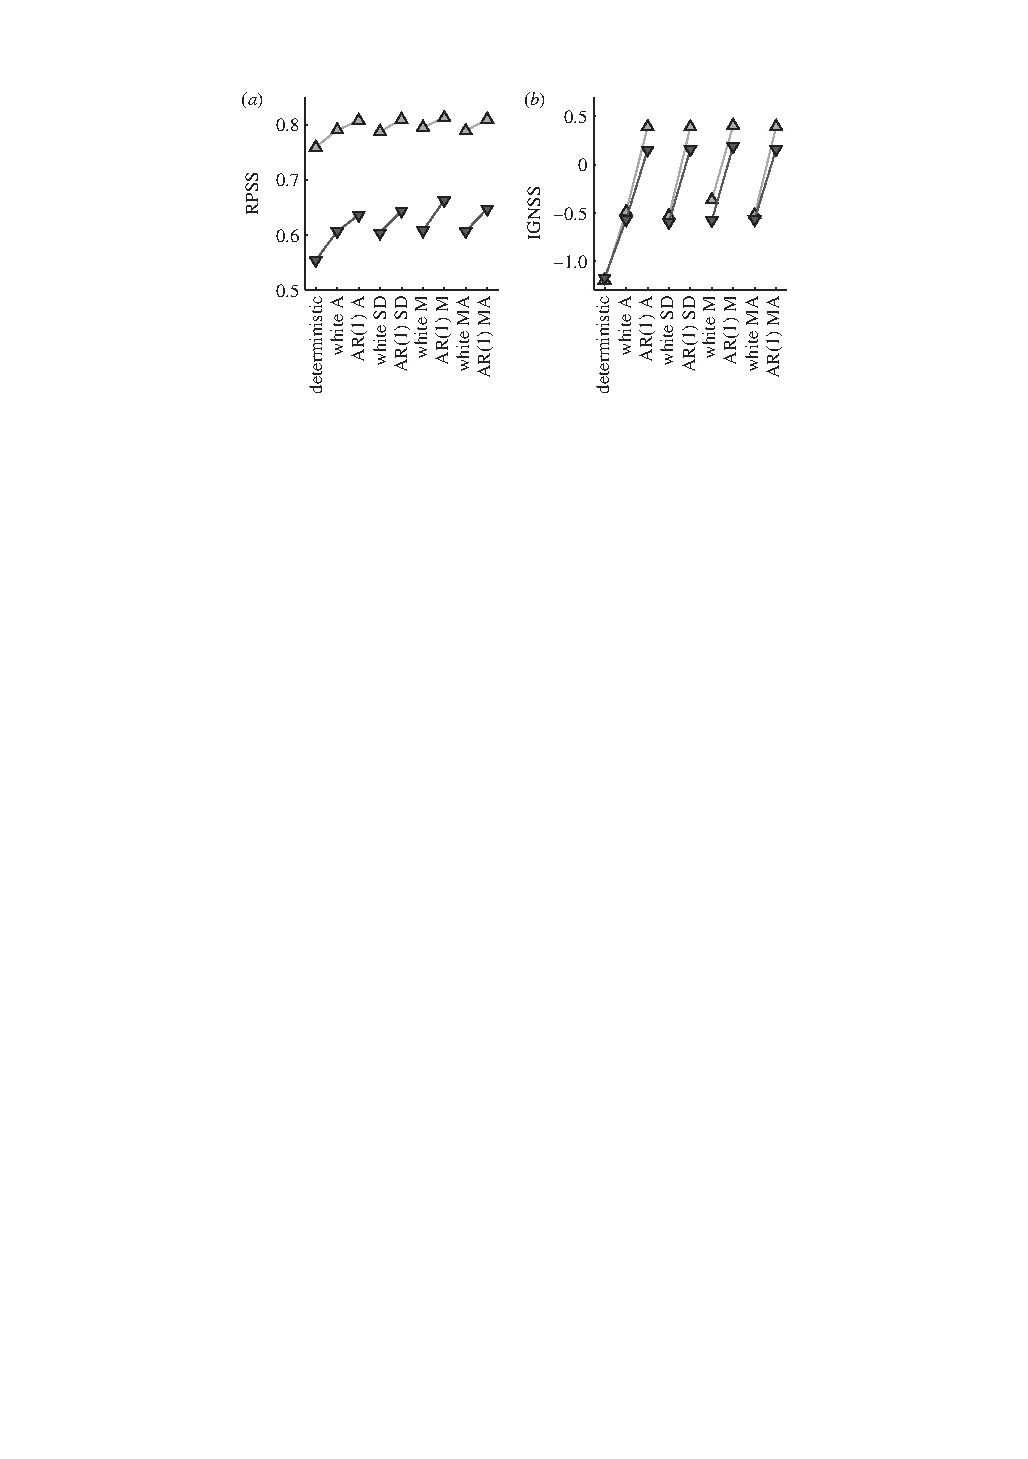
\includegraphics[width=0.6\linewidth]{figures/arnold2013_fig6.pdf}
    \caption{
        Reproduction of Figure 6 by \textcite{arnold2013}, showing a comparison
        of ensemble forecast skill for parametrisations with different types of
        noise. Skill is measured by the ranked probability skill score (RPSS;
        panel (a)) and ignorance skill score (IGNSS; panel (b)); higher values
        indicate better skill. The deterministic parametrisation is a cubic
        polynomial regression and added noise is either white or generated
        by an AR(1) process. Acronyms indicate the method used to introduce
        the noise; A = ``additive'', SD = ``state-dependent'' (noise standard
        deviation a linear function of $|X|$), M = ``multiplicative'' (SPPT)
        and MA = ``multiplicative and additive'' (noise standard deviation a
        linear function of $|P_\mathrm{det}(X)|$). Upright light grey triangles
        indicate results obtained under conditions of larger time scale
        separation ($c=10$ in \cref{eqn:l96}) and inverted dark grey triangles
        indicate smaller time scale separation ($c=4$). It is clear that
        schemes with white noise outperform deterministic ones, and schemes
        with AR(1) noise outperform whose with white noise.
    }
    \label{fig:arnold_fig6}
\end{figure}
\begin{figure}[H]
    \centering
    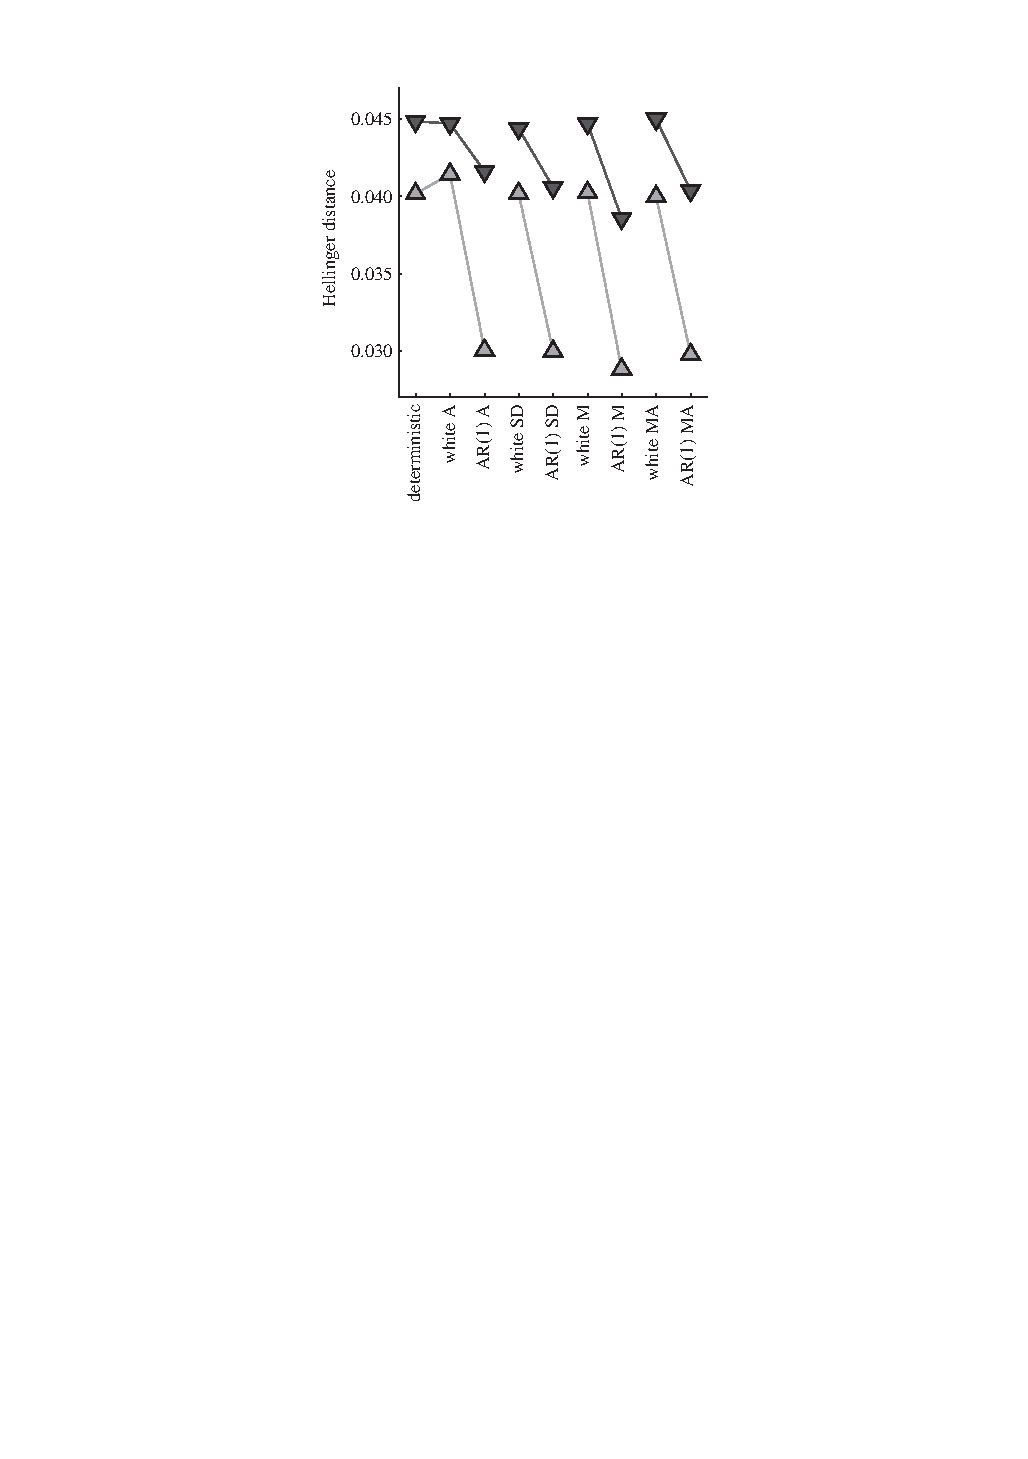
\includegraphics[width=0.4\linewidth]{figures/arnold2013_fig10.pdf}
    \caption{
        Reproduction of Figure 10 by \textcite{arnold2013}, comparing the
        accuracy with which parametrisations with different types of noise
        reproduce the true climatological PDFs of the resolved variables.
        Accuracy is measured by the Hellinger distance between the modelled
        and true PDFs; lower values indicate higher accuracy. The labels on
        the horizontal axis and the markers have the same meaning that they do
        in \cref{fig:arnold_fig6}. A clear improvement in accuracy is given
        by the schemes with AR(1) noise.
    }
    \label{fig:arnold_fig10}
\end{figure}

Some studies have obtained results that conflict with the aforementioned
consensus. Firstly \textcite{arnold2013} found no appreciable difference in
climatological PDF accuracy between their white noise and deterministic
schemes; this is evident in \cref{fig:arnold_fig10}. Analogously,
\textcite{christensen2015} similarly found no significant difference between
white noise and deterministic schemes in terms of their ability to reproduce
regime behaviour and predict the system's response to changes in the external
forcing parameter $F$. \textcite{gagne2020}, who constructed parametrisations
using generative adversarial networks, came to the unexpected conclusion that
using temporally correlated red noise may degrade the accuracy of ensemble
forecasts via an accumulation of noise-induced error and have little benefit
over white noise for climate prediction accuracy.

Several authors have postulated general interpretations of these results that
may be relevant to the parametrisation problem in dynamical systems beyond L96.
\textcite{arnold2013} attributed the apparent superiority of memory-based
parametrisations to a potential for subgrid-scale processes to influence the
resolved state on scales much larger than the grid scale at which the host
model is truncated; memory captures this spatial and temporal correlation or
persistence. \textcite{christensen2015} agreed with this assessment on the
basis of their results. They also argued that the persistence of correlated
noise is necessary to drive regime transitions that would otherwise be
underrepresented. Observing that stochastic parametrisation improved the
prediction of responses to changes in forcing, they further argued that
stochastic data-driven parametrisations are generally more likely to function
well in changed climate conditions outside the range of their training
datasets.


\subsection{Open questions and the case for more complex dynamical systems}
To conclude this section on data-driven parametrisation for L96, I will draw on
the key messages and conclusions in the literature to motivate further research
of the same kind in models of intermediate complexity.

Generally speaking, many parametrisation approaches of varying complexity have
shown promise when applied to L96; all the studies mentioned in
\cref{sec:l96_statmodels} were able to construct a scheme that reproduced the
properties of interest without egregious errors. Indeed, some of the more
recent and complex approaches have shown only marginal improvements over the
original regression-based approach introduced by \textcite{wilks2005}.
\textcite{gagne2020} attributed this to the simplicity of L96, which only
considers the evolution of a single field in one discrete spatial dimension.
There is hope that applying the L96 methods to dynamical systems with more
prognostic variables, spatial dimensions and degrees of freedom may reveal
deficiencies that were inconsequential in L96 and thus give researchers more
discriminative power in choosing approaches for application to full GCMs.

Several specific findings in L96 studies raise other questions that also
motivate a change of focus to more complex dynamical systems. The first is the
observation by \textcite{crommelin2008} that the advantage of their conditional
Markov chain parametrisation over the regression-based approach was greatest
under conditions of small time-scale separation and diminished with increasing
scale separation. \textcite{arnold2013} drew a similar conclusion regarding the
difference between stochastic and deterministic regression-based schemes. These
findings are consistent with the expectation that the net effect of
subgrid-scale processes should become increasingly unpredictable as resolution
increases and the size of the sample of small-scale events decreases (see
\cref{sec:traditional}). This is another piece of evidence that more realistic
fluid models, which do not have such a clean separation between ``resolved''
and ``unresolved'' variables, will be more discriminating and allow the best
approaches to show their full potential.

An open question of importance for real-world modelling concerns the extent to
which parametrisation schemes that result in accurate weather forecasts tend
can be expected to also produce accurate climate predictions
\parencite{christensen2019}. Another asks whether a scheme's offline
performance is a good indicator of its online performance once coupled into a
model. \textcite{gagne2020} addressed these questions by testing a collection
of GAN parametrisations with different predictors and types of noise (see
\cref{fig:gagne_fig11}), with the results suggesting an affirmative answer for
the former and a negative answer for the latter. The verification of these
conclusions would be a worthwhile goal for further research using other
dynamical systems. Other possible goals could be to more clearly assess
the ability of data-driven parametrisation schemes to adapt to unseen climate
conditions \parencite{christensen2015} and to explore and exploit the potential
for data-driven schemes to correct numerical errors in addition to modelling
unresolved processes \parencite{bhouri2023}.

\begin{figure}[ht]
    \centering
    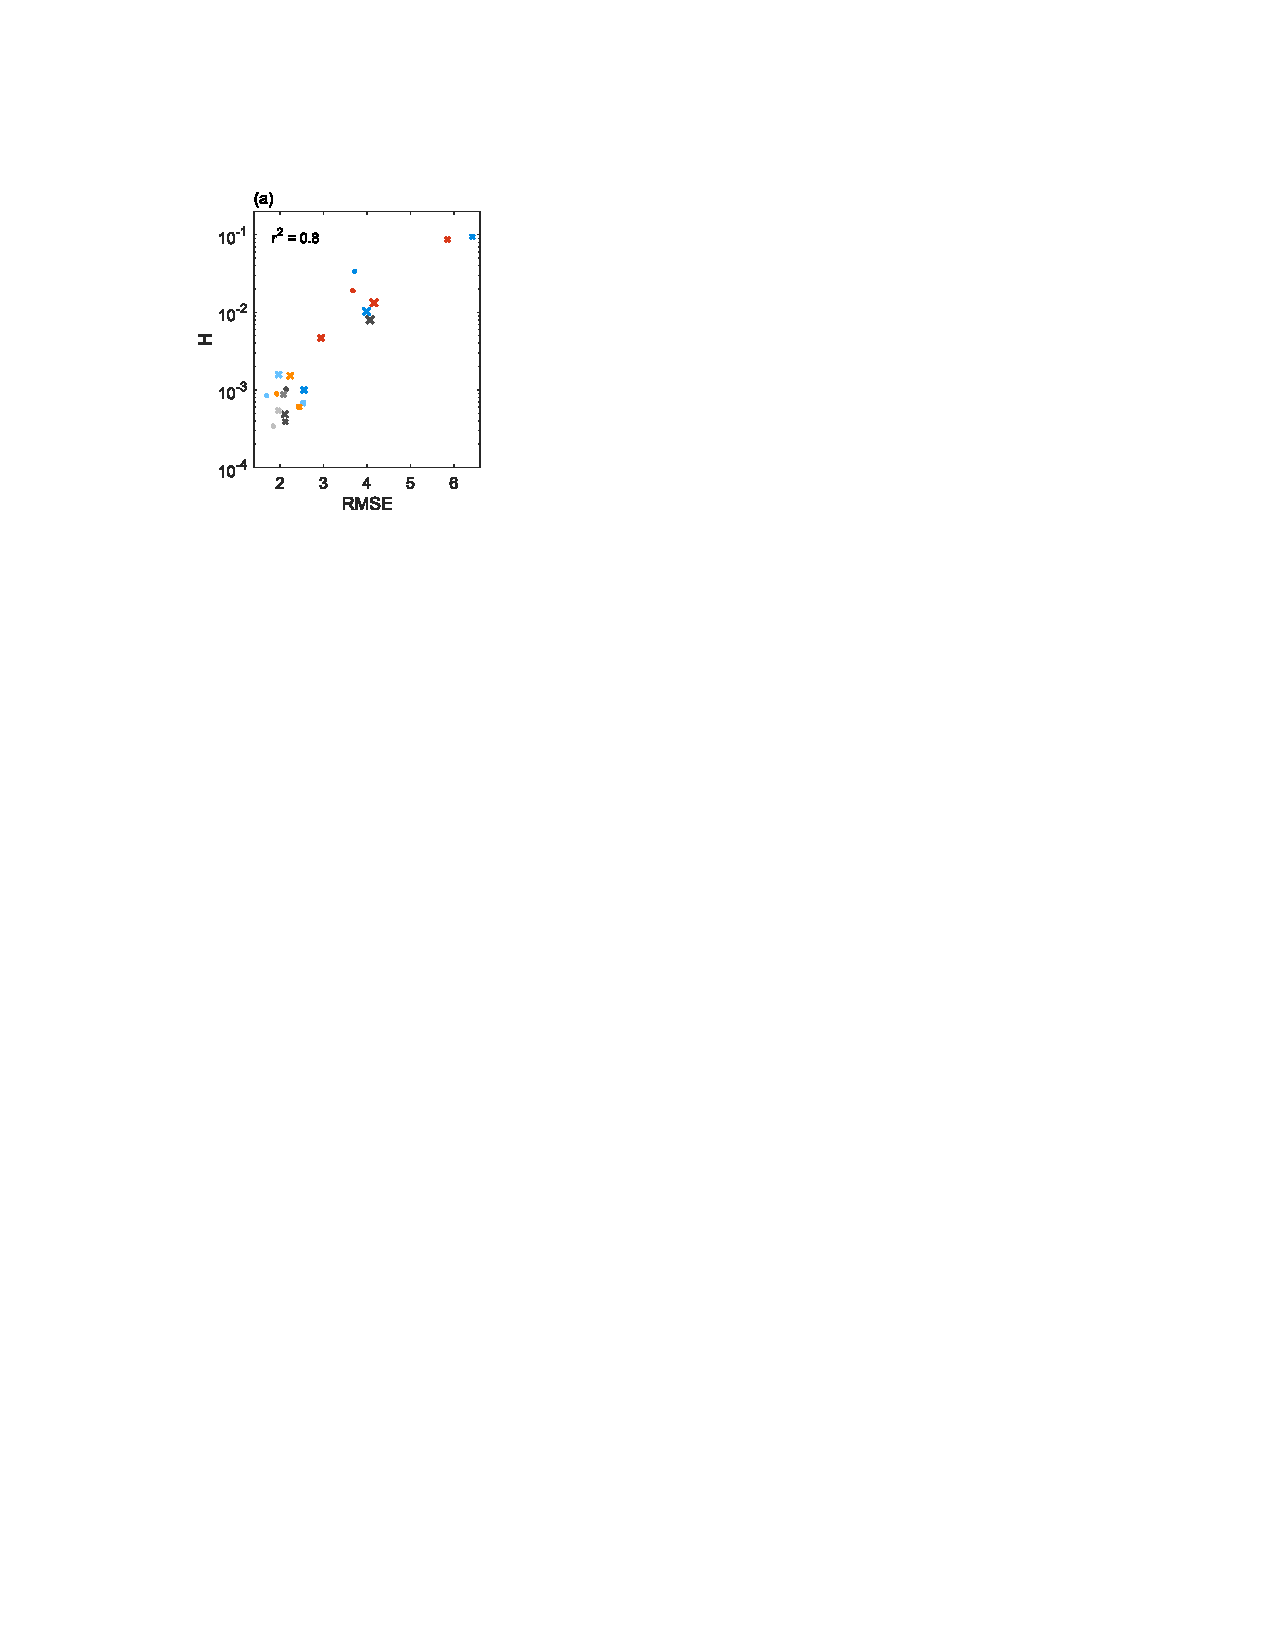
\includegraphics[width=0.3\linewidth]{figures/gagne_fig11a.pdf}%
    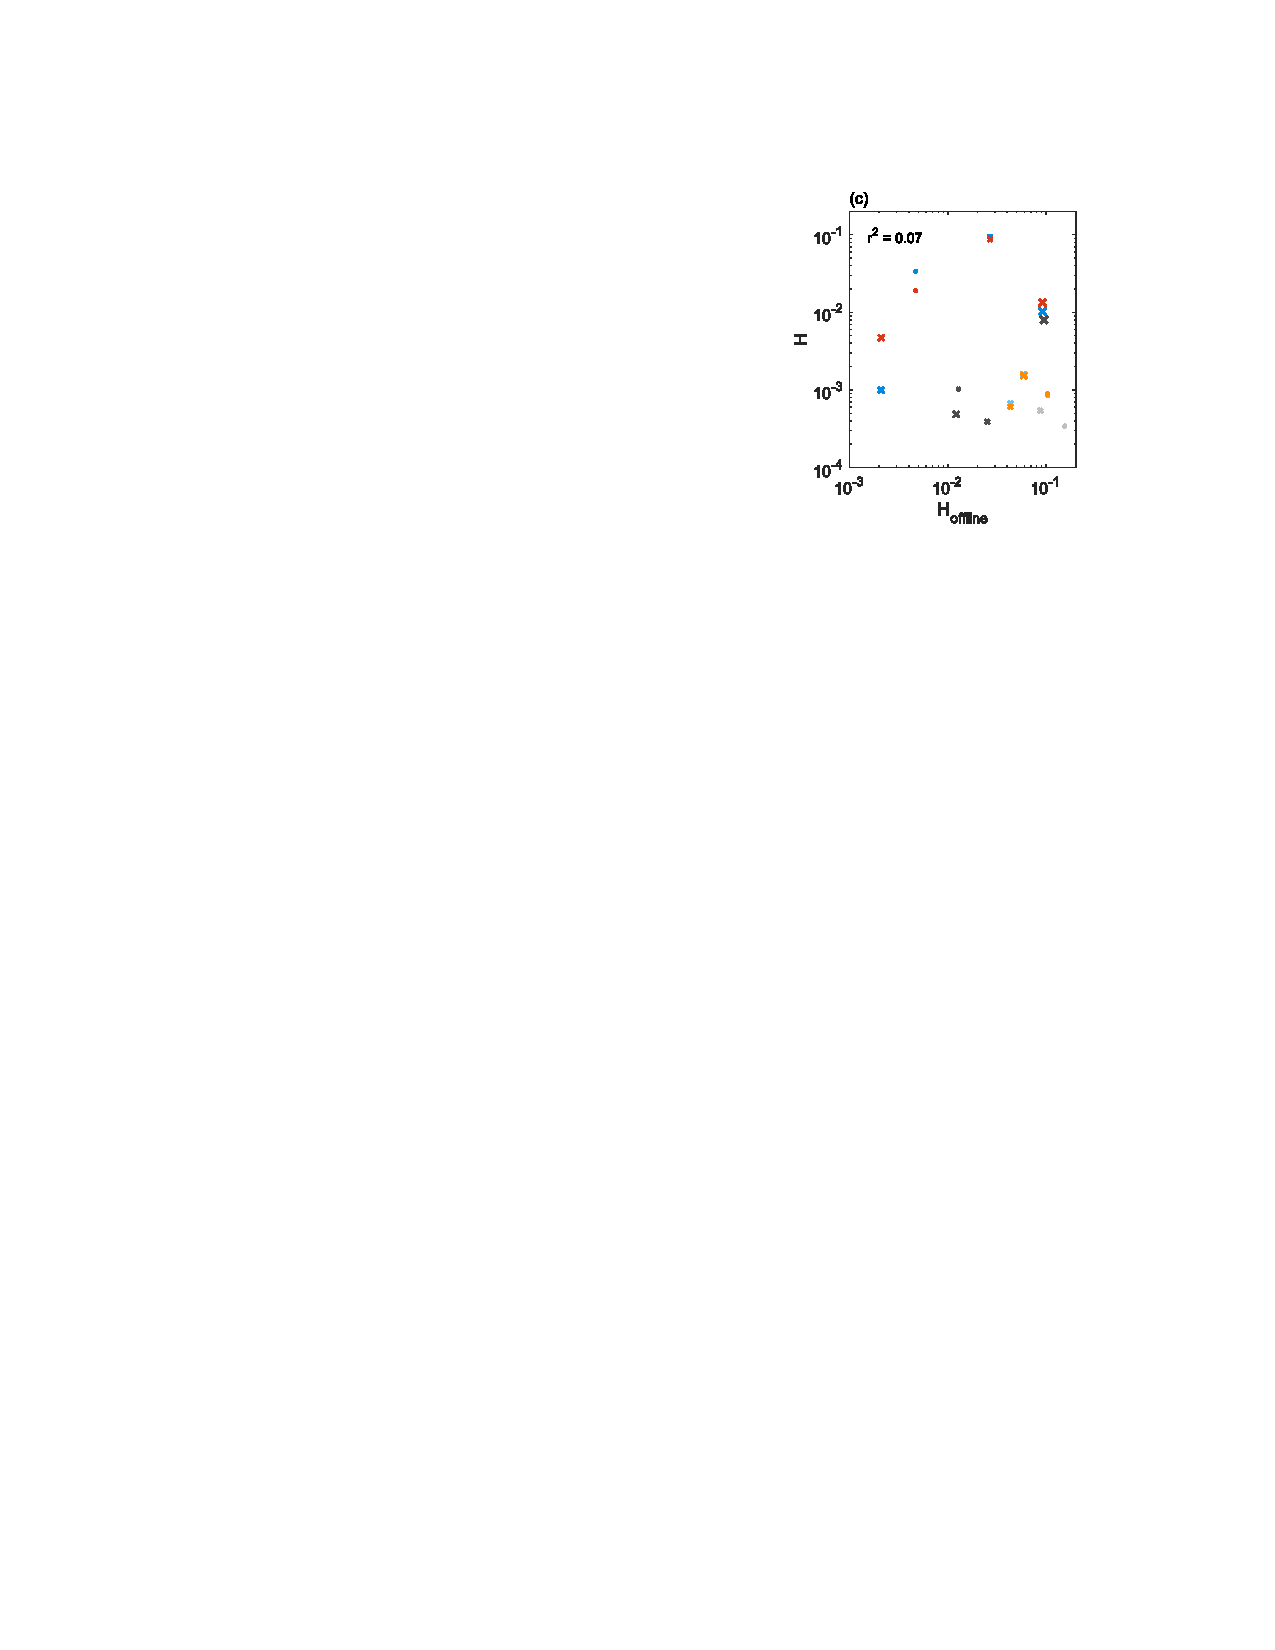
\includegraphics[width=0.3\linewidth]{figures/gagne_fig11c.pdf}
    \caption{
        Reproduction of Figures 11a and 11c by \textcite{gagne2020}.
        Panel (a) compares ensemble mean weather forecast accuracy
        (measured by RMSE) to climatological PDF accuracy (measured by the
        Hellinger distance $H$) for a collection of GAN parametrisations
        with different predictors and types of noise. Panel (c) performs a
        similar comparison with offline performance (measured by the Hellinger
        distance between the PDFs of the true and predicted tendencies)
        taking the place of RMSE.
    }
    \label{fig:gagne_fig11}
\end{figure}


\subsection{Beyond Lorenz '96}
The transition from L96 to more complex systems necessarily gives rise to
several technicalities that must be addressed. The most pressing of these is
the fact that increasing the number of degrees of freedom in the host model
will greatly increase the number of predictors available for parametrisations
to use. Models with more than one prognostic variable will also require
separate parametrisations for each one. Without judicious simplifications,
the problem of constructing a rigorous data-driven parametrisation will
quickly become intractable. \textcite{crommelin2008} give an insightful
discussion of this issue as it relates to Markov chain parametrisations.

Another complication is that the ``spatial'' dimension in L96 is
discrete, while the dynamical systems being parametrised in weather and
climate modelling (i.e., fluid flows) have continuous spatial
dimensions. While it is well established that there is little benefit in
using stochastic parametrisations with spatially correlated noise for
L96, spatial correlation is expected to be a much more important
consideration in spatially continuous systems \parencite{arnold2013}.
One might also ask whether it will be beneficial to construct spatially
nonlocal schemes where the tendency predicted at each point also depends on the
values of the large-scale variables at neighbouring points (potentially
capturing the gradients of these variables).


\clearpage
\section{Dynamical system case study: \rb{} convection}
In the final section of this review, I will present a case study on the
numerical modelling of \rb{} convection, arguing that it is an ideal
intermediate-complexity dynamical system for further parametrisation
development and testing. After reviewing the necessary preliminary material, I
will review the relevant literature to establish that under-resolved numerical
solutions of the system exhibit systematic errors that may be attributed to the
neglect of subgrid-scale dynamics. An understanding of the nature of these
errors will allow future work to use the \rb{} problem as a parametrisation
testbed analogous to L96, and inform the construction and testing of
data-driven schemes.


\subsection{Problem statement}
\rb{} convection is the motion of a fluid confined between two
horizontal isothermal plates, the temperature of the bottom plate being
higher than that of the top plate. The governing equations for the flow
follow from the Navier-Stokes equations of mass, energy and momentum
conservation. The reader is referred to \textcite{chandrasekhar1961} for
a detailed derivation; I summarise the assumptions and approximations
involved below.

The density, $\rho$, of the fluid is related to its temperature $T$ by
the linear equation of state
\[
    \rho = \rho_0 [1 - \alpha(T - T_0)],
\]
where $\alpha$ is the (constant) volume coefficient of thermal expansion and
$\rho_0$ and $T_0$ are the base-state density and temperature such that $\rho =
\rho_0$ when $T = T_0$. The key assumption is that density variations are small
($\alpha (T - T_0) \ll 1$), which allows the governing equations to be
simplified under the \emph{Boussinesq approximation}. The Boussinesq
approximation involves first writing the pressure, $p$, of the fluid as
\[
    p = p_0 - \rho_0 gz + p',
\]
where $p_0$ is an arbitrary constant, $g$ is the acceleration due to gravity
and $z$ is the vertical coordinate. $p'$ is the (time-varying) deviation from
a hydrostatically balanced background profile $p_0 - \rho_0 gz$
in which the upward pressure gradient force per unit volume $\rho_0 g$ cancels
the downward weight force per unit volume $-\rho_0 g$. Since
$\alpha (T - T_0) \ll 1$, density variations are neglected everywhere except
in their contribution to the weight force, leading to a net buoyant
(background pressure gradient plus weight) force per unit mass
\[
    \frac{\rho_0 - \rho}{\rho_0} g = \alpha (T - T_0) g.
\]

With these assumptions in mind, I adopt the governing equations as they
are derived by \textcite{chandrasekhar1961}:
\begin{alignat}{2}
    \label{eqn:dim_momentum}
    \pdiff{\vec{u}}{t} + \vec{u} \cdot \grad \vec{u}
        &= -\frac{1}{\rho_0} \grad p' + \alpha (T - T_0) g \uvec{z}
        + \nu \nabla^2 \vec{u}
    &\quad& \text{(momentum conservation),} \\
    \label{eqn:dim_energy}
    \pdiff{T}{t} + \vec{u} \cdot \grad T
        &= \kappa \nabla^2 T
    && \text{(energy conservation), and} \\
    \label{eqn:dim_incompressible}
    \grad \cdot \vec{u} &= 0
    && \text{(incompressibility).}
\end{alignat}
$\vec{u}$ is the fluid velocity, $t$ is time, $\uvec{z}$ is the upward
unit vector, $\nu$ is the (constant) kinematic viscosity and $\kappa$ is
the thermal diffusivity (also constant). Notice that the aforementioned
buoyancy term $\alpha (T - T_0) g$ appears on the right-hand side of
\cref{eqn:dim_momentum}.

The parametrisation test-bed developed in this work solves the governing
equations in a two-dimensional domain $(x,z) \in [0, d] \times [0, L]$, subject
to no-slip, isothermal boundary conditions on the top and bottom plates,
\begin{alignat}{3}
    \label{eqn:dim_bc_bot}
    \vec{u} &= \vec{0}, &\quad T &= T_0 + \frac{\delta T}{2}
    &\qquad& \text{at } z = 0 \text{ and} \\
    \label{eqn:dim_bc_top}
    \vec{u} &= \vec{0}, &\quad T &= T_0 - \frac{\delta T}{2}
    &\qquad& \text{at } z = d,
\end{alignat}
and periodic boundary conditions in the horizontal,
\begin{alignat}{2}
    \label{eqn:dim_bc_sides}
    \vec{u}(x=0) &= \vec{u}(x=L) &\quad \text{and} \quad T(x=0) &= T(x=L).
\end{alignat}
$\delta T$ is the constant temperature difference between the plates.

\subsection{Nondimensionalisation and scale analysis}
It is helpful to nondimensionalise the governing equations
\crefrange{eqn:dim_momentum}{eqn:dim_bc_sides}; this is not only useful for
numerical work but also gives insight into the different flow regimes that are
possible. A range of nondimensionalisations are used in fluid dynamics
literature; I adopt a common one \parencite[see,
e.g.,][]{grotzbach1983,ouertatani2008,stevens2010} which is suitable for the
turbulent convective regime.

For low-viscosity, turbulent flow, a suitable time scale is the
\emph{free-fall time} $t_0$, which is the time for a fluid element with
constant temperature $T = T_0 - \delta T$ to fall from the top plate to
the bottom plate under the influence of buoyancy ($-g \alpha \delta T$)
alone. It is simple to show that
\[
    t_0 \sim \left( \frac{d}{g \alpha \delta T} \right)^{1/2},
\]
ignoring a factor of $\sqrt{2}$. The obvious length and temperature
scales are the plate separation $d$ and temperature difference $\delta T$,
respectively.

Making the substitutions $p'/\rho_0 \to \pi$ and $T - T_0 \to \theta$
in \crefrange{eqn:dim_momentum}{eqn:dim_bc_sides} and expressing all
variables in units of $t_0$, $d$ and $\delta T$ leads to the dimensionless
equations
\begin{align}
    \label{eqn:momentum}
    \pdiff{\vec{u}}{t} + \vec{u} \cdot \grad \vec{u}
        &= -\grad \pi + \left( \frac{\prandtl}{\rayleigh}\right)^{1/2}
        \nabla^2 \vec{u} + \theta \uvec{z}, \\
    \label{eqn:energy}
    \pdiff{\theta}{t} + \vec{u} \cdot \grad \theta
        &= (\rayleigh\,\prandtl)^{-1/2} \, \nabla^2 \theta, \quad \text{and} \\
    \label{eqn:incompressible}
    \grad \cdot \vec{u} &= 0,
\end{align}
with boundary conditions
\begin{gather}
\begin{alignat}{3}
    \label{eqn:bc_bot}
    \vec{u} &= \vec{0}, &\quad \theta &= +\frac{1}{2}
    &\qquad& \text{at } z = 0, \\
    \label{eqn:bc_top}
    \vec{u} &= \vec{0}, &\quad \theta &= -\frac{1}{2}
    &\qquad& \text{at } z = 1,
\end{alignat} \\
\begin{alignat}{2}
    \label{eqn:bc_sides}
    \vec{u}(x=0) &= \vec{u}(x=\Gamma)
    &\quad \text{and} \quad \theta(x=0) &= \theta(x=\Gamma).
\end{alignat}
\end{gather}
There are three dimensionless parameters: the aspect ratio of the domain
\[
    \Gamma \equiv \frac{L}{d},
\]
the \emph{Prandtl number}
\[
    \prandtl \equiv \frac{\nu}{\kappa}
\]
which measures the relative importance of viscosity (momentum diffusivity)
and thermal diffusivity, and the \emph{Rayleigh number}
\[
    \rayleigh \equiv \frac{g \alpha d^3 \delta T}{\kappa \nu}.
\]
The Rayleigh number can be interpreted as the ratio of the time scale for
thermal transport by conduction to the time scale for
thermal transport by convection. It determines the importance of diffusion for the evolution of
$\vec{u}$ and $\theta$; inspection of \cref{eqn:momentum,eqn:energy} indicates
that low $\rayleigh$ implies strong diffusion and high $\rayleigh$ weak
diffusion. Detailed theoretical analysis of the governing equations (see, e.g.,
\textcite{chandrasekhar1961} and the seminal work by \textcite{rayleigh1916})
reveals that there exists a critical Rayleigh number (dependent on boundary
conditions but of order $\SI{e3}{}$), below which the equations have a stable
equilibrium with the fluid at rest and a linear conductive temperature profile.
Above the critical value, the equilibrium is unstable and small perturbations
lead to the formation of a regular series of steady, rotating convection cells.
If the Rayleigh number is increased much further (\textcite{le_quere1991} cites
$\rayleigh \approx \SI{2e8}{}$), the solution becomes unsteady and increasingly
turbulent. This work is concerned with the turbulent regime, since Rayleigh
numbers for atmospheric deep moist convection can be as large as $\SI{e22}{}$
\parencite{chilla2012}.

\subsection{Thermal properties}
Two more definitions are necessary before proceeding.
First, the Nusselt number measures the rate of
(vertical) heat transport across a horizontal plane at height $z$, normalised
by the purely conductive rate that would exist if the fluid were at rest
\parencite{verzicco1999}. Following \textcite{chilla2012}, I use the definition
(before nondimensionalisation)
\begin{equation}
    \label{eqn:dim_nusselt}
    \nusselt(z,t) \equiv \frac{
        \langle wT \rangle_{A,t}
        - \kappa \partial \langle T \rangle_{A,t} / \partial z
    }{
        \kappa \delta T / d
    }
\end{equation}
where $\langle \cdot \rangle_{A,t}$ denotes averaging over time and the
horizontal plane at height $z$, and $w = \vec{u} \cdot \uvec{z}$ is the
vertical velocity. The rate of heat transport in the numerator has two terms:
advection $\langle wT \rangle_{A,t}$ and conduction $-\kappa \partial \langle T
\rangle_{A,t} / \partial z$. The denominator $\kappa \delta T / d$ is the rate
of heat transport for a linear conductive temperature profile with the fluid at
rest.

Another important quantity is the thickness $\delta_T$ of the \emph{thermal
boundary layer} at each plate where large temperature gradients exist.
\textcite{chilla2012} define $\delta_T$ as follows: if, on average, the fluid
temperature changes with height from $+\delta T/2$ at the lower plate to $0$
(the mean value in the well-mixed interior) over a distance $\delta_T$, then
\[
    \left. \pdiff{\langle T \rangle_{A,t}}{z} \right|_{z=0}
        \approx -\frac{\delta T}{2 \delta_T}.
\]
But if one considers the definition of the Nusselt number
\cref{eqn:dim_nusselt} at $z=0$, the advection term $\langle wT \rangle_{A,t}$
vanishes due to the $\vec{u} = \vec{0}$ boundary condition and
\[
    \nusselt(z=0) = -\frac{d}{\delta T}
        \left. \pdiff{\langle T \rangle_{A,t}}{z} \right|_{z=0}.
\]
Thus,
\begin{equation}
    \label{eqn:thermal_bl}
    \delta_T = \frac{d}{2\,\nusselt(z=0)}.
\end{equation}


\subsection{Resolution dependence of numerical solutions}
% s.sherwood: Might be important to further explain here that you will regard
% this as the ("warts and all") dynamical system you want to emulate at a
% coarser representation.  This avoids the issue of whether this hig-res is a
% perfect solution of the fluid equations or not (it doesn't have to be,
% although for robustness we want it to be relatively insensitive to small
% changes in dx).
The first basic requirement for a parametrisation testbed is a reasonably accurate high-resolution model to treat as truth. The next requirement is a truncated coarse model which posesses systematic biases relative to truth that might reasonably be improved by parametrising the unresolved subgrid-scale dynamics. In this section, I review relevant literature on numerical solutions of the \rb{} problem with the aim of
establishing the nature of the biases that might be expected. Practically, the following questions must be answered:
\begin{itemize}
    \item What resolution is necessary for a converged solution?
    \item Which quantities are most sensitive to insufficient resolution?
\end{itemize}


\subsubsection{Theoretical resolution requirements for accurate simulations}%
\label{sec:res_requirements}

% resolution in general, Grotzbach condition.
\textcite{grotzbach1983} is recognised as the first to formulate resolution
requirements for accurate simulations of \rb{} convection
\parencite{chilla2012,scheel2013}. He identified separate constraints on the
mean (i.e., averaged in each spatial direction) grid spacing and the vertical
spacing near the plates; I first discuss the former.
\citeauthor{grotzbach1983} reasoned that a numerical model that neglects
subgrid-scale effects must have a geometric mean grid spacing $h = (\Delta x
\Delta y \Delta z)^{1/3}$ such that
\begin{equation}
    \label{eqn:grotzbach}
    h \leq \pi \eta = \pi \left(
        \frac{\nu^3}{\langle \epsilon \rangle}
    \right)^{1/4}
\end{equation}
where $\eta \equiv (\nu^3/\langle \epsilon \rangle)^{1/4}$ is the \emph{Kolmogorov length}, the
universal smallest relevant length scale for general turbulent flow, and
$\langle \epsilon \rangle$ is the spatial and temporal average of the kinetic
energy dissipation rate defined by
\begin{equation}
    \label{eqn:kinetic_dissipation}
    \epsilon(\vec{x}, t) \equiv \frac{\nu}{2} \sum_{ij} \left(
        \pdiff{u_i}{x_j} + \pdiff{u_j}{x_i}
    \right)^2
\end{equation}
\parencite{chilla2012}. The inequality \cref{eqn:grotzbach} between $h$ and $\eta$ can be
understood using the Nyquist-Shannon theorem, which states that a
sampling frequency $f \geq k/\pi$ is needed to unambiguously reconstruct
a signal with maximum wavenumber $k$; substituting $f = 1/h$, $k =
1/\eta$ leads to the claimed relation.

% resolution near plates, number of points.
\citeauthor{grotzbach1983} recognised that the above reasoning was only valid
for the mean grid spacing; large gradients in temperature and velocity near the
top and bottom plates require finer resolution in those regions. The notion of
nearness can be formalised using the thermal boundary layer thickness
\cref{eqn:thermal_bl}, and one asks how many grid points are necessary in this
layer. \citeauthor{grotzbach1983} did not give a theoretical argument to derive
this number but claimed that 3 points are sufficient for turbulent flows.
\textcite{shishkina2010} presented a theoretical argument based on the
(experimentally and numerically justified) assumption of laminar
\emph{Prandtl-Blasius} flow conditions in the boundary layer and were able to
calculate the minimum number of grid points (e.g., 9 for $\rayleigh =
\SI{2e9}{}$ and $\prandtl = 0.7$). The results agreed with criteria derived in
previous numerical experiments. Importantly, the results of
\citeauthor{shishkina2010} allow \emph{a priori} determination of vertical
resolution requirements, potentially bypassing the time-consuming and expensive
process of iteratively running simulations, checking their convergence and
updating the resolution.

\subsubsection{
    Resolution-dependence tests and consequences of under-resolution}%
\label{sec:res_tests}

Performing numerical experiments for a 3D fluid layer,
\citeauthor{grotzbach1983} found that RMS velocity and Nusselt number were
the most sensitive quantities to insufficient mean grid spacing, but even
they increased ``only slightly'' above the values obtained from well-resolved
simulations. He concluded that condition \cref{eqn:grotzbach} was overly
restrictive and recommended (for $\prandtl > 0.59$) the simplified,
approximate version
\[ % is this necessary?
    h \lesssim 5.23 \, \prandtl^{-1/4} \rayleigh^{-0.3205}.
\]
Later work also supports the finding that the Nusselt number is
sensitive to under-resolution. Even studying only steady-state convective
solutions at moderate Rayleigh number, \textcite{le_quere1991} found that the
maximum and minimum Nusselt numbers were most sensitive to changes in
resolution and had the largest uncertainty among existing benchmark solutions.
% ouertatani: common to use Nu as convergence test
Other studies have used the convergence of the Nusselt number as an indicator
that the spatial resolution is sufficient to produce an accurate solution
\parencite{ouertatani2008}.

\textcite{stevens2010} performed 3D simulations in a finite cylindrical cavity
with the aim of reconciling the apparent disagreement between the Nusselt
numbers in previous numerical studies and experimental observations. They found
that agreement with experiment could be achieved, but only by using a much
higher resolution than the previous studies. They offered the physical
explanation that horizontally under-resolved simulations produce insufficient
thermal diffusion, leading to systematic overestimation of the buoyancy of
convective plumes near the side-walls of the cylinder; this results in Nusselt
numbers that exceed experimentally observed values. This led them to conclude
that the two criteria of \textcite{grotzbach1983}---for mean grid spacing
and for the vertical spacing near the upper and lower plates---are not
independent; the definition $h = (\Delta x \Delta y \Delta z)^{1/3}$ in
\cref{eqn:grotzbach} allows the horizontal spacing to remain relatively
coarse near the plates, provided the vertical spacing is small. Since
fine horizontal resolution is also necessary to accurately capture
the dynamics of the thin plumes, they proposed that \cref{eqn:grotzbach} be
applied with $h = \max(\Delta x, \Delta y, \Delta z)$ instead.

% kooij: Nu may not be best indicator
Some more recent work, however, casts doubt on the notion that the Nusselt
number is sensitive to under-resolution and that its convergence is a good
indicator that the flow is well-resolved. In assessing the performance of
several published computational fluid dynamics codes on the \rb{} problem in a
cylindrical cavity, \textcite{kooij2018} identified one higher-order code that
reproduced the theoretically predicted scaling of $\nusselt$ as a function of
$\rayleigh$ even when the flow was deliberately under-resolved. On the other
hand, the presence of numerical artefacts in the instantaneous temperature
field near the bottom plate was a clear indicator of insufficient resolution.


% scheel: dissipation rates sensitive
\textcite{scheel2013} performed similar high-resolution simulations for
a cylindrical cavity and also found that the Nusselt number, among other
global transport properties, were ``fairly insensitive to insufficient
resolution, as long as the mean Kolmogorov length [was] resolved'' (i.e.,
\cref{eqn:grotzbach} was satisfied). However, they found that the horizontally
averaged or local kinetic energy dissipation rate
\cref{eqn:kinetic_dissipation} and the corresponding thermal dissipation rate
\begin{equation}
    \label{eqn:thermal_dissipation}
    \epsilon_T(\vec{x}, t) \equiv \kappa \sum_i \left(\pdiff{T}{x_i}\right)^2
\end{equation}
were much more sensitive, with their convergence requiring even stricter
conditions than \cref{eqn:grotzbach}.

In summary, conditions on the mean grid spacing and number of grid points in the thermal boundary layer exist to guide high-resolution simulations. It is known that the Nusselt number and kinetic and thermal dissipatiom rates are sensitive to under-resolution, so the statistics of these quantities could serve as metrics for evaluating parametrisation performance.


\clearpage
\section{Summary}

\clearpage
\emergencystretch=5em
\printbibliography
\end{document}
